% Options for packages loaded elsewhere
\PassOptionsToPackage{unicode}{hyperref}
\PassOptionsToPackage{hyphens}{url}
%
\documentclass[
]{book}
\usepackage{lmodern}
\usepackage{amsmath}
\usepackage{ifxetex,ifluatex}
\ifnum 0\ifxetex 1\fi\ifluatex 1\fi=0 % if pdftex
  \usepackage[T1]{fontenc}
  \usepackage[utf8]{inputenc}
  \usepackage{textcomp} % provide euro and other symbols
  \usepackage{amssymb}
\else % if luatex or xetex
  \usepackage{unicode-math}
  \defaultfontfeatures{Scale=MatchLowercase}
  \defaultfontfeatures[\rmfamily]{Ligatures=TeX,Scale=1}
\fi
% Use upquote if available, for straight quotes in verbatim environments
\IfFileExists{upquote.sty}{\usepackage{upquote}}{}
\IfFileExists{microtype.sty}{% use microtype if available
  \usepackage[]{microtype}
  \UseMicrotypeSet[protrusion]{basicmath} % disable protrusion for tt fonts
}{}
\makeatletter
\@ifundefined{KOMAClassName}{% if non-KOMA class
  \IfFileExists{parskip.sty}{%
    \usepackage{parskip}
  }{% else
    \setlength{\parindent}{0pt}
    \setlength{\parskip}{6pt plus 2pt minus 1pt}}
}{% if KOMA class
  \KOMAoptions{parskip=half}}
\makeatother
\usepackage{xcolor}
\IfFileExists{xurl.sty}{\usepackage{xurl}}{} % add URL line breaks if available
\IfFileExists{bookmark.sty}{\usepackage{bookmark}}{\usepackage{hyperref}}
\hypersetup{
  pdftitle={회귀모형 R 실습},
  pdfauthor={서울시립대학교 통계학과 이용희},
  hidelinks,
  pdfcreator={LaTeX via pandoc}}
\urlstyle{same} % disable monospaced font for URLs
\usepackage{color}
\usepackage{fancyvrb}
\newcommand{\VerbBar}{|}
\newcommand{\VERB}{\Verb[commandchars=\\\{\}]}
\DefineVerbatimEnvironment{Highlighting}{Verbatim}{commandchars=\\\{\}}
% Add ',fontsize=\small' for more characters per line
\usepackage{framed}
\definecolor{shadecolor}{RGB}{248,248,248}
\newenvironment{Shaded}{\begin{snugshade}}{\end{snugshade}}
\newcommand{\AlertTok}[1]{\textcolor[rgb]{0.94,0.16,0.16}{#1}}
\newcommand{\AnnotationTok}[1]{\textcolor[rgb]{0.56,0.35,0.01}{\textbf{\textit{#1}}}}
\newcommand{\AttributeTok}[1]{\textcolor[rgb]{0.77,0.63,0.00}{#1}}
\newcommand{\BaseNTok}[1]{\textcolor[rgb]{0.00,0.00,0.81}{#1}}
\newcommand{\BuiltInTok}[1]{#1}
\newcommand{\CharTok}[1]{\textcolor[rgb]{0.31,0.60,0.02}{#1}}
\newcommand{\CommentTok}[1]{\textcolor[rgb]{0.56,0.35,0.01}{\textit{#1}}}
\newcommand{\CommentVarTok}[1]{\textcolor[rgb]{0.56,0.35,0.01}{\textbf{\textit{#1}}}}
\newcommand{\ConstantTok}[1]{\textcolor[rgb]{0.00,0.00,0.00}{#1}}
\newcommand{\ControlFlowTok}[1]{\textcolor[rgb]{0.13,0.29,0.53}{\textbf{#1}}}
\newcommand{\DataTypeTok}[1]{\textcolor[rgb]{0.13,0.29,0.53}{#1}}
\newcommand{\DecValTok}[1]{\textcolor[rgb]{0.00,0.00,0.81}{#1}}
\newcommand{\DocumentationTok}[1]{\textcolor[rgb]{0.56,0.35,0.01}{\textbf{\textit{#1}}}}
\newcommand{\ErrorTok}[1]{\textcolor[rgb]{0.64,0.00,0.00}{\textbf{#1}}}
\newcommand{\ExtensionTok}[1]{#1}
\newcommand{\FloatTok}[1]{\textcolor[rgb]{0.00,0.00,0.81}{#1}}
\newcommand{\FunctionTok}[1]{\textcolor[rgb]{0.00,0.00,0.00}{#1}}
\newcommand{\ImportTok}[1]{#1}
\newcommand{\InformationTok}[1]{\textcolor[rgb]{0.56,0.35,0.01}{\textbf{\textit{#1}}}}
\newcommand{\KeywordTok}[1]{\textcolor[rgb]{0.13,0.29,0.53}{\textbf{#1}}}
\newcommand{\NormalTok}[1]{#1}
\newcommand{\OperatorTok}[1]{\textcolor[rgb]{0.81,0.36,0.00}{\textbf{#1}}}
\newcommand{\OtherTok}[1]{\textcolor[rgb]{0.56,0.35,0.01}{#1}}
\newcommand{\PreprocessorTok}[1]{\textcolor[rgb]{0.56,0.35,0.01}{\textit{#1}}}
\newcommand{\RegionMarkerTok}[1]{#1}
\newcommand{\SpecialCharTok}[1]{\textcolor[rgb]{0.00,0.00,0.00}{#1}}
\newcommand{\SpecialStringTok}[1]{\textcolor[rgb]{0.31,0.60,0.02}{#1}}
\newcommand{\StringTok}[1]{\textcolor[rgb]{0.31,0.60,0.02}{#1}}
\newcommand{\VariableTok}[1]{\textcolor[rgb]{0.00,0.00,0.00}{#1}}
\newcommand{\VerbatimStringTok}[1]{\textcolor[rgb]{0.31,0.60,0.02}{#1}}
\newcommand{\WarningTok}[1]{\textcolor[rgb]{0.56,0.35,0.01}{\textbf{\textit{#1}}}}
\usepackage{longtable,booktabs}
\usepackage{calc} % for calculating minipage widths
% Correct order of tables after \paragraph or \subparagraph
\usepackage{etoolbox}
\makeatletter
\patchcmd\longtable{\par}{\if@noskipsec\mbox{}\fi\par}{}{}
\makeatother
% Allow footnotes in longtable head/foot
\IfFileExists{footnotehyper.sty}{\usepackage{footnotehyper}}{\usepackage{footnote}}
\makesavenoteenv{longtable}
\usepackage{graphicx}
\makeatletter
\def\maxwidth{\ifdim\Gin@nat@width>\linewidth\linewidth\else\Gin@nat@width\fi}
\def\maxheight{\ifdim\Gin@nat@height>\textheight\textheight\else\Gin@nat@height\fi}
\makeatother
% Scale images if necessary, so that they will not overflow the page
% margins by default, and it is still possible to overwrite the defaults
% using explicit options in \includegraphics[width, height, ...]{}
\setkeys{Gin}{width=\maxwidth,height=\maxheight,keepaspectratio}
% Set default figure placement to htbp
\makeatletter
\def\fps@figure{htbp}
\makeatother
\setlength{\emergencystretch}{3em} % prevent overfull lines
\providecommand{\tightlist}{%
  \setlength{\itemsep}{0pt}\setlength{\parskip}{0pt}}
\setcounter{secnumdepth}{5}
%----- my options----------------
\usepackage[hangul]{kotex}
\usepackage{bm}
\usepackage{fullpage}

\newcommand{\pardiff}[2]{\frac{\partial #1}{\partial #2 }}
\newcommand{\pardiffl}[2]{{\partial #1}/{\partial #2 }}
\newcommand{\pardiffd}[2]{\frac{\partial^2 #1}{\partial #2^t \partial #2 }}
\newcommand{\pardiffdd}[3]{\frac{\partial^2 #1}{\partial #2 \partial #3 }}
\newcommand{\norm}[1]{\left\lVert#1\right\rVert}
\newcommand{\hatmat}{\bm X ({\bm X}^t {\bm X} )^{-1} {\bm X}^t}
\newcommand{\hatmatt}[1]{\bm X_{#1} ({\bm X}_{#1}^t {\bm X}_{#1})^{-1} {\bm X}_{#1}^t}

%--------- from bookdown.org --------------

\usepackage{booktabs}


\usepackage{framed,color}
\definecolor{shadecolor}{RGB}{248,248,248}

\renewcommand{\textfraction}{0.05}
\renewcommand{\topfraction}{0.8}
\renewcommand{\bottomfraction}{0.8}
\renewcommand{\floatpagefraction}{0.75}

\renewenvironment{quote}{\begin{VF}}{\end{VF}}
\let\oldhref\href
\renewcommand{\href}[2]{#2\footnote{\url{#1}}}

\makeatletter
\newenvironment{kframe}{%
\medskip{}
\setlength{\fboxsep}{.8em}
 \def\at@end@of@kframe{}%
 \ifinner\ifhmode%
  \def\at@end@of@kframe{\end{minipage}}%
  \begin{minipage}{\columnwidth}%
 \fi\fi%
 \def\FrameCommand##1{\hskip\@totalleftmargin \hskip-\fboxsep
 \colorbox{shadecolor}{##1}\hskip-\fboxsep
     % There is no \\@totalrightmargin, so:
     \hskip-\linewidth \hskip-\@totalleftmargin \hskip\columnwidth}%
 \MakeFramed {\advance\hsize-\width
   \@totalleftmargin\z@ \linewidth\hsize
   \@setminipage}}%
 {\par\unskip\endMakeFramed%
 \at@end@of@kframe}
\makeatother

\makeatletter

\@ifundefined{Shaded}{
}{\renewenvironment{Shaded}{\begin{kframe}}{\end{kframe}}}
\makeatother

\newenvironment{rmdblock}[1]
  {
  \begin{itemize}
  \renewcommand{\labelitemi}{
    \raisebox{-.7\height}[0pt][0pt]{
      {\setkeys{Gin}{width=3em,keepaspectratio}\includegraphics{images/#1}}
    }
  }
  \setlength{\fboxsep}{1em}
  \begin{kframe}
  \item
  }
  {
  \end{kframe}
  \end{itemize}
  }
  
\newenvironment{rmdnote}
  {\begin{rmdblock}{note}}
  {\end{rmdblock}}
  
\newenvironment{rmdcaution}
  {\begin{rmdblock}{caution}}
  {\end{rmdblock}}
  
\newenvironment{rmdimportant}
  {\begin{rmdblock}{important}}
  {\end{rmdblock}}
  
\newenvironment{rmdtip}
  {\begin{rmdblock}{tip}}
  {\end{rmdblock}}
  
\newenvironment{rmdwarning}
  {\begin{rmdblock}{warning}}
  {\end{rmdblock}}
  


\usepackage{makeidx}
\makeindex

\urlstyle{tt}

\usepackage{amsthm}
\makeatletter
 \def\thm@space@setup{%
   \thm@preskip=8pt plus 2pt minus 4pt
   \thm@postskip=\thm@preskip
}
\makeatother

\frontmatter
\usepackage{booktabs}
\usepackage{longtable}
\usepackage{array}
\usepackage{multirow}
\usepackage{wrapfig}
\usepackage{float}
\usepackage{colortbl}
\usepackage{pdflscape}
\usepackage{tabu}
\usepackage{threeparttable}
\usepackage{threeparttablex}
\usepackage[normalem]{ulem}
\usepackage{makecell}
\usepackage{xcolor}
\ifluatex
  \usepackage{selnolig}  % disable illegal ligatures
\fi
\usepackage[]{natbib}
\bibliographystyle{apalike}

\title{회귀모형 R 실습}
\author{서울시립대학교 통계학과 이용희}
\date{2021-04-13}

\begin{document}
\maketitle

{
\setcounter{tocdepth}{1}
\tableofcontents
}
\hypertarget{preface}{%
\chapter*{Preface}\label{preface}}


이 책은 일반 선형모형에 대한 R 프로그램과 결과에 대하여 설명합니다.

다음과 같은 R 패키지가 필요합니다.

\begin{verbatim}
library(ggplot2)
library(dplyr)
library(tidyr)
library(kableExtra)
library(regbook)
library(ellipse)
library(car)
library(MASS)
library(Matrix)
\end{verbatim}

\begin{rmdimportant}
이 책에서 사용된 기호, 표기법, 프로그램의 규칙과 쓰임은 다음과 같습니다.

\begin{itemize}
\tightlist
\item
  스칼라(scalar)와 일변량 확률변수는 일반적으로 보통 글씨체의 소문자로 표기한다. 특별한 이유가 있는 경우 대문자로 표시할 것이다.
\item
  벡터, 행렬, 다변량 확률벡터는 굵은 글씨체로 표기한다.
\item
  통계 프로그램은 \texttt{R}을 이용하였다. 각 예제에 사용된 \texttt{R} 프로그램은 코드 상자를 열면 나타난다.
\item
  통계 프로그램은 \texttt{R}에 대한 기초는 저자의 홈페이지에 있는 \href{https://ilovedata.github.io/computing/}{안내 사이트}에서 먼저 학습할 것을 권장한다.
\end{itemize}
\end{rmdimportant}

\mainmatter

\hypertarget{chapter03}{%
\chapter{중회귀분석}\label{chapter03}}

예제 3.3에 나온 중고차 가격자료를 이용한 R 실습입니다.
\#\#

\hypertarget{uxc911uxace0uxcc28-uxc790uxb8cc}{%
\section{중고차 자료}\label{uxc911uxace0uxcc28-uxc790uxb8cc}}

\begin{Shaded}
\begin{Highlighting}[]
\FunctionTok{head}\NormalTok{(usedcars)}
\end{Highlighting}
\end{Shaded}

\begin{verbatim}
##   price year mileage   cc automatic
## 1   790   78  133462 1998         1
## 2  1380   39   33000 2000         1
## 3   270  109  120000 1800         0
## 4  1190   20   69727 1999         1
## 5   590   70  112000 2000         0
## 6  1120   58   39106 1998         1
\end{verbatim}

\hypertarget{uxc0b0uxc810uxb3c4-uxd589uxb82c}{%
\section{산점도 행렬}\label{uxc0b0uxc810uxb3c4-uxd589uxb82c}}

\begin{Shaded}
\begin{Highlighting}[]
\FunctionTok{pairs}\NormalTok{(usedcars)}
\end{Highlighting}
\end{Shaded}

\includegraphics{lmpractice_files/figure-latex/unnamed-chunk-5-1.pdf}

\hypertarget{uxc911uxd68cuxadc0-uxbaa8uxd615uxc758-uxc801uxd569}{%
\section{중회귀 모형의 적합}\label{uxc911uxd68cuxadc0-uxbaa8uxd615uxc758-uxc801uxd569}}

\begin{Shaded}
\begin{Highlighting}[]
\NormalTok{fit0 }\OtherTok{\textless{}{-}} \FunctionTok{lm}\NormalTok{(price }\SpecialCharTok{\textasciitilde{}}\NormalTok{ year }\SpecialCharTok{+}\NormalTok{ mileage }\SpecialCharTok{+}\NormalTok{ cc }\SpecialCharTok{+}\NormalTok{ automatic, usedcars)}
\end{Highlighting}
\end{Shaded}

계획행렬은 다음과 같이 구할 수 있다.

\begin{Shaded}
\begin{Highlighting}[]
\FunctionTok{model.matrix}\NormalTok{(fit0)}
\end{Highlighting}
\end{Shaded}

\begin{verbatim}
##    (Intercept) year mileage   cc automatic
## 1            1   78  133462 1998         1
## 2            1   39   33000 2000         1
## 3            1  109  120000 1800         0
## 4            1   20   69727 1999         1
## 5            1   70  112000 2000         0
## 6            1   58   39106 1998         1
## 7            1   53   95935 1800         1
## 8            1   68  120000 1800         0
## 9            1   15   20215 1798         1
## 10           1   96  140000 1800         0
## 11           1   63   68924 1998         1
## 12           1   82   90000 2000         0
## 13           1   76   81279 1998         0
## 14           1   17   24070 1798         1
## 15           1   38   40000 2000         0
## 16           1   46   56887 1832         1
## 17           1   95   91216 1997         1
## 18           1   37   48680 1998         1
## 19           1   68    8000 2000         0
## 20           1   41   60634 1835         1
## 21           1   69  114131 1998         1
## 22           1   71   75000 1800         0
## 23           1   99  124417 1998         1
## 24           1  129  130000 1800         0
## 25           1   57   77559 1997         1
## 26           1  107   75216 1838         1
## 27           1   45   52000 2000         0
## 28           1   80   58000 2000         1
## 29           1  113  134500 1800         0
## 30           1   41   80000 2000         0
## attr(,"assign")
## [1] 0 1 2 3 4
\end{verbatim}

\texttt{fit0} 에 저장된 결과를 다음과 같이 함수 \texttt{str}을 이용하여 볼 수 있다.

\begin{Shaded}
\begin{Highlighting}[]
\FunctionTok{str}\NormalTok{(fit0)}
\end{Highlighting}
\end{Shaded}

\begin{verbatim}
## List of 12
##  $ coefficients : Named num [1:5] 525.28696 -5.79964 -0.00226 0.38879 165.31263
##   ..- attr(*, "names")= chr [1:5] "(Intercept)" "year" "mileage" "cc" ...
##  $ residuals    : Named num [1:30] 76.98 212.69 -51.4 -4.01 -53.45 ...
##   ..- attr(*, "names")= chr [1:30] "1" "2" "3" "4" ...
##  $ effects      : Named num [1:30] -4407 -1434 -369 -229 419 ...
##   ..- attr(*, "names")= chr [1:30] "(Intercept)" "year" "mileage" "cc" ...
##  $ rank         : int 5
##  $ fitted.values: Named num [1:30] 713 1167 321 1194 643 ...
##   ..- attr(*, "names")= chr [1:30] "1" "2" "3" "4" ...
##  $ assign       : int [1:5] 0 1 2 3 4
##  $ qr           :List of 5
##   ..$ qr   : num [1:30, 1:5] -5.477 0.183 0.183 0.183 0.183 ...
##   .. ..- attr(*, "dimnames")=List of 2
##   .. .. ..$ : chr [1:30] "1" "2" "3" "4" ...
##   .. .. ..$ : chr [1:5] "(Intercept)" "year" "mileage" "cc" ...
##   .. ..- attr(*, "assign")= int [1:5] 0 1 2 3 4
##   ..$ qraux: num [1:5] 1.18 1.18 1.08 1.03 1.26
##   ..$ pivot: int [1:5] 1 2 3 4 5
##   ..$ tol  : num 1e-07
##   ..$ rank : int 5
##   ..- attr(*, "class")= chr "qr"
##  $ df.residual  : int 25
##  $ xlevels      : Named list()
##  $ call         : language lm(formula = price ~ year + mileage + cc + automatic, data = usedcars)
##  $ terms        :Classes 'terms', 'formula'  language price ~ year + mileage + cc + automatic
##   .. ..- attr(*, "variables")= language list(price, year, mileage, cc, automatic)
##   .. ..- attr(*, "factors")= int [1:5, 1:4] 0 1 0 0 0 0 0 1 0 0 ...
##   .. .. ..- attr(*, "dimnames")=List of 2
##   .. .. .. ..$ : chr [1:5] "price" "year" "mileage" "cc" ...
##   .. .. .. ..$ : chr [1:4] "year" "mileage" "cc" "automatic"
##   .. ..- attr(*, "term.labels")= chr [1:4] "year" "mileage" "cc" "automatic"
##   .. ..- attr(*, "order")= int [1:4] 1 1 1 1
##   .. ..- attr(*, "intercept")= int 1
##   .. ..- attr(*, "response")= int 1
##   .. ..- attr(*, ".Environment")=<environment: R_GlobalEnv> 
##   .. ..- attr(*, "predvars")= language list(price, year, mileage, cc, automatic)
##   .. ..- attr(*, "dataClasses")= Named chr [1:5] "numeric" "numeric" "numeric" "numeric" ...
##   .. .. ..- attr(*, "names")= chr [1:5] "price" "year" "mileage" "cc" ...
##  $ model        :'data.frame':   30 obs. of  5 variables:
##   ..$ price    : int [1:30] 790 1380 270 1190 590 1120 815 450 1290 420 ...
##   ..$ year     : int [1:30] 78 39 109 20 70 58 53 68 15 96 ...
##   ..$ mileage  : int [1:30] 133462 33000 120000 69727 112000 39106 95935 120000 20215 140000 ...
##   ..$ cc       : int [1:30] 1998 2000 1800 1999 2000 1998 1800 1800 1798 1800 ...
##   ..$ automatic: int [1:30] 1 1 0 1 0 1 1 0 1 0 ...
##   ..- attr(*, "terms")=Classes 'terms', 'formula'  language price ~ year + mileage + cc + automatic
##   .. .. ..- attr(*, "variables")= language list(price, year, mileage, cc, automatic)
##   .. .. ..- attr(*, "factors")= int [1:5, 1:4] 0 1 0 0 0 0 0 1 0 0 ...
##   .. .. .. ..- attr(*, "dimnames")=List of 2
##   .. .. .. .. ..$ : chr [1:5] "price" "year" "mileage" "cc" ...
##   .. .. .. .. ..$ : chr [1:4] "year" "mileage" "cc" "automatic"
##   .. .. ..- attr(*, "term.labels")= chr [1:4] "year" "mileage" "cc" "automatic"
##   .. .. ..- attr(*, "order")= int [1:4] 1 1 1 1
##   .. .. ..- attr(*, "intercept")= int 1
##   .. .. ..- attr(*, "response")= int 1
##   .. .. ..- attr(*, ".Environment")=<environment: R_GlobalEnv> 
##   .. .. ..- attr(*, "predvars")= language list(price, year, mileage, cc, automatic)
##   .. .. ..- attr(*, "dataClasses")= Named chr [1:5] "numeric" "numeric" "numeric" "numeric" ...
##   .. .. .. ..- attr(*, "names")= chr [1:5] "price" "year" "mileage" "cc" ...
##  - attr(*, "class")= chr "lm"
\end{verbatim}

\hypertarget{uxd68cuxadc0uxacc4uxc218uxc758-uxcd94uxc815uxacfc-uxacb0uxc815uxacc4uxc218}{%
\section{회귀계수의 추정과 결정계수}\label{uxd68cuxadc0uxacc4uxc218uxc758-uxcd94uxc815uxacfc-uxacb0uxc815uxacc4uxc218}}

함수 \texttt{summary} 는 각 계수의 추정값과 가설 \(H_0: \beta_i=0\)에 대한 t-검정 결과를 보여준다.
또한 결정계수 \(R^2\)도 구해준다.

\begin{Shaded}
\begin{Highlighting}[]
\FunctionTok{summary}\NormalTok{(fit0)}
\end{Highlighting}
\end{Shaded}

\begin{verbatim}
## 
## Call:
## lm(formula = price ~ year + mileage + cc + automatic, data = usedcars)
## 
## Residuals:
##     Min      1Q  Median      3Q     Max 
## -177.35  -63.91   -0.99   70.34  212.69 
## 
## Coefficients:
##               Estimate Std. Error t value Pr(>|t|)    
## (Intercept)  5.253e+02  3.998e+02   1.314 0.200823    
## year        -5.800e+00  9.283e-01  -6.247 1.55e-06 ***
## mileage     -2.263e-03  7.211e-04  -3.138 0.004324 ** 
## cc           3.888e-01  2.022e-01   1.923 0.065958 .  
## automatic    1.653e+02  3.986e+01   4.147 0.000339 ***
## ---
## Signif. codes:  0 '***' 0.001 '**' 0.01 '*' 0.05 '.' 0.1 ' ' 1
## 
## Residual standard error: 101.1 on 25 degrees of freedom
## Multiple R-squared:  0.9045, Adjusted R-squared:  0.8892 
## F-statistic: 59.21 on 4 and 25 DF,  p-value: 2.184e-12
\end{verbatim}

각 회귀 계수에 대한 신뢰구간은 함수 \texttt{confint}로 구할 수 있다.

\begin{Shaded}
\begin{Highlighting}[]
\FunctionTok{confint}\NormalTok{(fit0)}
\end{Highlighting}
\end{Shaded}

\begin{verbatim}
##                     2.5 %        97.5 %
## (Intercept) -2.981256e+02  1.348699e+03
## year        -7.711605e+00 -3.887669e+00
## mileage     -3.748021e-03 -7.776672e-04
## cc          -2.763072e-02  8.052054e-01
## automatic    8.322275e+01  2.474025e+02
\end{verbatim}

공동 신뢰영역은 패키지 \texttt{ellipse} 에 있는 함수 \texttt{ellipse}를 이용해서 다음과 같이 그릴 수 있다.

\begin{Shaded}
\begin{Highlighting}[]
\FunctionTok{plot}\NormalTok{(ellipse}\SpecialCharTok{::}\FunctionTok{ellipse}\NormalTok{(fit0, }\AttributeTok{level =} \FloatTok{0.90}\NormalTok{), }\AttributeTok{type =} \StringTok{\textquotesingle{}l\textquotesingle{}}\NormalTok{)}
\end{Highlighting}
\end{Shaded}

\includegraphics{lmpractice_files/figure-latex/unnamed-chunk-11-1.pdf}

\begin{Shaded}
\begin{Highlighting}[]
\FunctionTok{plot}\NormalTok{(ellipse}\SpecialCharTok{::}\FunctionTok{ellipse}\NormalTok{(fit0, }\AttributeTok{which =} \FunctionTok{c}\NormalTok{(}\StringTok{\textquotesingle{}year\textquotesingle{}}\NormalTok{, }\StringTok{\textquotesingle{}mileage\textquotesingle{}}\NormalTok{), }\AttributeTok{level =} \FloatTok{0.90}\NormalTok{), }\AttributeTok{type =} \StringTok{\textquotesingle{}l\textquotesingle{}}\NormalTok{)}
\FunctionTok{points}\NormalTok{(fit0}\SpecialCharTok{$}\NormalTok{coefficients[}\StringTok{\textquotesingle{}year\textquotesingle{}}\NormalTok{], fit0}\SpecialCharTok{$}\NormalTok{coefficients[}\StringTok{\textquotesingle{}mileage\textquotesingle{}}\NormalTok{])}
\end{Highlighting}
\end{Shaded}

\includegraphics{lmpractice_files/figure-latex/unnamed-chunk-12-1.pdf}
\#\# 분산분석

\begin{Shaded}
\begin{Highlighting}[]
\FunctionTok{anova}\NormalTok{(fit0)}
\end{Highlighting}
\end{Shaded}

\begin{verbatim}
## Analysis of Variance Table
## 
## Response: price
##           Df  Sum Sq Mean Sq  F value    Pr(>F)    
## year       1 2056608 2056608 201.2036 1.841e-13 ***
## mileage    1  135864  135864  13.2919 0.0012228 ** 
## cc         1   52409   52409   5.1273 0.0324794 *  
## automatic  1  175828  175828  17.2018 0.0003389 ***
## Residuals 25  255538   10222                       
## ---
## Signif. codes:  0 '***' 0.001 '**' 0.01 '*' 0.05 '.' 0.1 ' ' 1
\end{verbatim}

\hypertarget{uxc608uxce21uxac12}{%
\section{예측값}\label{uxc608uxce21uxac12}}

반응변수에 대한 예측값 \(\hat {\bm y} = \bm X \hat {\bm \beta}\)는 함수 \texttt{redict}를 이용한다.

\begin{Shaded}
\begin{Highlighting}[]
\FunctionTok{predict}\NormalTok{(fit0)}
\end{Highlighting}
\end{Shaded}

\begin{verbatim}
##         1         2         3         4         5         6         7         8 
##  713.0214 1167.3146  321.4025 1194.0114  643.4485 1042.5270  865.9501  559.1876 
##         9        10        11        12        13        14        15        16 
## 1256.9013  351.5409  946.0553  623.6355  677.3900 1236.5788  991.9617 1007.3483 
##        17        18        19        20        21        22        23        24 
##  709.6348 1142.6549  890.3836 1029.0340  808.9611  643.6167  611.6964  182.7813 
##        25        26        27        28        29        30 
##  960.9247  614.4275  924.2101  872.9584  265.3927  884.0490
\end{verbatim}

새로운 자료에 대한 예측값 \(\widehat { E(y|x)}\)은 다음과 같이 데이터프레임을 만들고 예측한다.

\begin{Shaded}
\begin{Highlighting}[]
\NormalTok{nw }\OtherTok{\textless{}{-}} \FunctionTok{data.frame}\NormalTok{(}\AttributeTok{year=}\DecValTok{60}\NormalTok{, }\AttributeTok{mileage=}\DecValTok{10000}\NormalTok{, }\AttributeTok{cc=}\DecValTok{200}\NormalTok{, }\AttributeTok{automatic=}\DecValTok{1}\NormalTok{)}
\NormalTok{nw}
\end{Highlighting}
\end{Shaded}

\begin{verbatim}
##   year mileage  cc automatic
## 1   60   10000 200         1
\end{verbatim}

\begin{Shaded}
\begin{Highlighting}[]
\FunctionTok{predict}\NormalTok{(fit0, }\AttributeTok{newdata=}\NormalTok{nw, }\AttributeTok{interval=}\StringTok{"confidence"}\NormalTok{)}
\end{Highlighting}
\end{Shaded}

\begin{verbatim}
##        fit       lwr      upr
## 1 397.7504 -342.6272 1138.128
\end{verbatim}

새로운 관측값에 대항 예측은 다음과 같이 한다.

\begin{Shaded}
\begin{Highlighting}[]
\FunctionTok{predict}\NormalTok{(fit0, }\AttributeTok{newdata=}\NormalTok{nw, }\AttributeTok{interval=}\StringTok{"prediction"}\NormalTok{)}
\end{Highlighting}
\end{Shaded}

\begin{verbatim}
##        fit       lwr      upr
## 1 397.7504 -371.3501 1166.851
\end{verbatim}

\hypertarget{uxc794uxcc28-uxbd84uxc11d}{%
\section{잔차 분석}\label{uxc794uxcc28-uxbd84uxc11d}}

\begin{Shaded}
\begin{Highlighting}[]
\FunctionTok{plot}\NormalTok{(fit0)}
\end{Highlighting}
\end{Shaded}

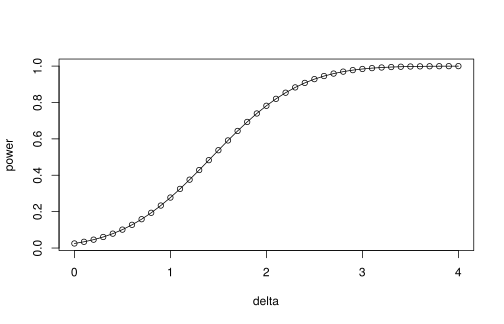
\includegraphics{lmpractice_files/figure-latex/unnamed-chunk-17-1.pdf} \includegraphics{lmpractice_files/figure-latex/unnamed-chunk-17-2.pdf} \includegraphics{lmpractice_files/figure-latex/unnamed-chunk-17-3.pdf} \includegraphics{lmpractice_files/figure-latex/unnamed-chunk-17-4.pdf}

\hypertarget{chapter04}{%
\chapter{모형의 진단과 수정}\label{chapter04}}

예제 3.3에 나온 중고차 가격자료를 이용한 R 실습입니다.

\hypertarget{uxc21cuxcc28uxc81cuxacf1uxd569}{%
\section{순차제곱합}\label{uxc21cuxcc28uxc81cuxacf1uxd569}}

순차제곱합은 모형에 들어가는 변수의 순서에 따라서 제곱합이 틀려진다.

다음의 예를 보면 두 모형이 같은 변수들로 적합되지만 순서가 달라지면 순차제곱합이 다르다.

\begin{Shaded}
\begin{Highlighting}[]
\NormalTok{model1 }\OtherTok{\textless{}{-}}\NormalTok{ price }\SpecialCharTok{\textasciitilde{}}\NormalTok{ year }\SpecialCharTok{+}\NormalTok{ mileage }\SpecialCharTok{+}\NormalTok{ cc }\SpecialCharTok{+}\NormalTok{ automatic}
\NormalTok{model2 }\OtherTok{\textless{}{-}}\NormalTok{ price }\SpecialCharTok{\textasciitilde{}}\NormalTok{ mileage }\SpecialCharTok{+}\NormalTok{ automatic }\SpecialCharTok{+}\NormalTok{ cc }\SpecialCharTok{+}\NormalTok{ year}
\NormalTok{fit1 }\OtherTok{\textless{}{-}} \FunctionTok{lm}\NormalTok{(model1, usedcars)}
\NormalTok{fit2 }\OtherTok{\textless{}{-}} \FunctionTok{lm}\NormalTok{(model2, usedcars)}
\FunctionTok{anova}\NormalTok{(fit1)}
\end{Highlighting}
\end{Shaded}

\begin{verbatim}
## Analysis of Variance Table
## 
## Response: price
##           Df  Sum Sq Mean Sq  F value    Pr(>F)    
## year       1 2056608 2056608 201.2036 1.841e-13 ***
## mileage    1  135864  135864  13.2919 0.0012228 ** 
## cc         1   52409   52409   5.1273 0.0324794 *  
## automatic  1  175828  175828  17.2018 0.0003389 ***
## Residuals 25  255538   10222                       
## ---
## Signif. codes:  0 '***' 0.001 '**' 0.01 '*' 0.05 '.' 0.1 ' ' 1
\end{verbatim}

\begin{Shaded}
\begin{Highlighting}[]
\FunctionTok{anova}\NormalTok{(fit2)}
\end{Highlighting}
\end{Shaded}

\begin{verbatim}
## Analysis of Variance Table
## 
## Response: price
##           Df  Sum Sq Mean Sq  F value    Pr(>F)    
## mileage    1 1637355 1637355 160.1870 2.274e-12 ***
## automatic  1  341741  341741  33.4335 5.006e-06 ***
## cc         1   42683   42683   4.1758   0.05168 .  
## year       1  398929  398929  39.0283 1.552e-06 ***
## Residuals 25  255538   10222                       
## ---
## Signif. codes:  0 '***' 0.001 '**' 0.01 '*' 0.05 '.' 0.1 ' ' 1
\end{verbatim}

하지만 회귀계수의 추정량은 동일하다.

\begin{Shaded}
\begin{Highlighting}[]
\FunctionTok{summary}\NormalTok{(fit1)}
\end{Highlighting}
\end{Shaded}

\begin{verbatim}
## 
## Call:
## lm(formula = model1, data = usedcars)
## 
## Residuals:
##     Min      1Q  Median      3Q     Max 
## -177.35  -63.91   -0.99   70.34  212.69 
## 
## Coefficients:
##               Estimate Std. Error t value Pr(>|t|)    
## (Intercept)  5.253e+02  3.998e+02   1.314 0.200823    
## year        -5.800e+00  9.283e-01  -6.247 1.55e-06 ***
## mileage     -2.263e-03  7.211e-04  -3.138 0.004324 ** 
## cc           3.888e-01  2.022e-01   1.923 0.065958 .  
## automatic    1.653e+02  3.986e+01   4.147 0.000339 ***
## ---
## Signif. codes:  0 '***' 0.001 '**' 0.01 '*' 0.05 '.' 0.1 ' ' 1
## 
## Residual standard error: 101.1 on 25 degrees of freedom
## Multiple R-squared:  0.9045, Adjusted R-squared:  0.8892 
## F-statistic: 59.21 on 4 and 25 DF,  p-value: 2.184e-12
\end{verbatim}

\begin{Shaded}
\begin{Highlighting}[]
\FunctionTok{summary}\NormalTok{(fit2)}
\end{Highlighting}
\end{Shaded}

\begin{verbatim}
## 
## Call:
## lm(formula = model2, data = usedcars)
## 
## Residuals:
##     Min      1Q  Median      3Q     Max 
## -177.35  -63.91   -0.99   70.34  212.69 
## 
## Coefficients:
##               Estimate Std. Error t value Pr(>|t|)    
## (Intercept)  5.253e+02  3.998e+02   1.314 0.200823    
## mileage     -2.263e-03  7.211e-04  -3.138 0.004324 ** 
## automatic    1.653e+02  3.986e+01   4.147 0.000339 ***
## cc           3.888e-01  2.022e-01   1.923 0.065958 .  
## year        -5.800e+00  9.283e-01  -6.247 1.55e-06 ***
## ---
## Signif. codes:  0 '***' 0.001 '**' 0.01 '*' 0.05 '.' 0.1 ' ' 1
## 
## Residual standard error: 101.1 on 25 degrees of freedom
## Multiple R-squared:  0.9045, Adjusted R-squared:  0.8892 
## F-statistic: 59.21 on 4 and 25 DF,  p-value: 2.184e-12
\end{verbatim}

\hypertarget{uxd3b8uxc81cuxacf1uxd569}{%
\section{편제곱합}\label{uxd3b8uxc81cuxacf1uxd569}}

편제곱합은 다른 변수들로 보정된 제곱합으로 순서에 관계없이 일정하다.패키지 \texttt{car} 에 있는 함수 \texttt{Anova} 를 사용하면
편제곱합을 구할 수 있다.

\begin{Shaded}
\begin{Highlighting}[]
\FunctionTok{Anova}\NormalTok{(fit1, }\AttributeTok{type=}\StringTok{"III"}\NormalTok{)}
\end{Highlighting}
\end{Shaded}

\begin{verbatim}
## Anova Table (Type III tests)
## 
## Response: price
##             Sum Sq Df F value    Pr(>F)    
## (Intercept)  17645  1  1.7262 0.2008228    
## year        398929  1 39.0283 1.552e-06 ***
## mileage     100649  1  9.8467 0.0043244 ** 
## cc           37794  1  3.6975 0.0659577 .  
## automatic   175828  1 17.2018 0.0003389 ***
## Residuals   255538 25                      
## ---
## Signif. codes:  0 '***' 0.001 '**' 0.01 '*' 0.05 '.' 0.1 ' ' 1
\end{verbatim}

\begin{Shaded}
\begin{Highlighting}[]
\FunctionTok{Anova}\NormalTok{(fit2, }\AttributeTok{type=}\StringTok{"III"}\NormalTok{)}
\end{Highlighting}
\end{Shaded}

\begin{verbatim}
## Anova Table (Type III tests)
## 
## Response: price
##             Sum Sq Df F value    Pr(>F)    
## (Intercept)  17645  1  1.7262 0.2008228    
## mileage     100649  1  9.8467 0.0043244 ** 
## automatic   175828  1 17.2018 0.0003389 ***
## cc           37794  1  3.6975 0.0659577 .  
## year        398929  1 39.0283 1.552e-06 ***
## Residuals   255538 25                      
## ---
## Signif. codes:  0 '***' 0.001 '**' 0.01 '*' 0.05 '.' 0.1 ' ' 1
\end{verbatim}

\hypertarget{uxbd80uxbd84-f-uxac80uxc815}{%
\section{부분 F 검정}\label{uxbd80uxbd84-f-uxac80uxc815}}

배기량(cc)에 대항 계수가 0인지 검정해보자.

\[ H_0: ~ \beta_k =0 \]

하나의 계수에 대한 검정은 분산분석 표의 t-검정으로도 가능하며 결과는 동일하다.

\begin{Shaded}
\begin{Highlighting}[]
\NormalTok{fullmodel }\OtherTok{\textless{}{-}}\NormalTok{ price }\SpecialCharTok{\textasciitilde{}}\NormalTok{ year }\SpecialCharTok{+}\NormalTok{ mileage }\SpecialCharTok{+}\NormalTok{ cc }\SpecialCharTok{+}\NormalTok{ automatic}
\NormalTok{reducemodel1 }\OtherTok{\textless{}{-}}\NormalTok{ price }\SpecialCharTok{\textasciitilde{}}\NormalTok{ year }\SpecialCharTok{+}\NormalTok{ mileage }\SpecialCharTok{+}\NormalTok{ automatic}
\NormalTok{fitfull }\OtherTok{\textless{}{-}} \FunctionTok{lm}\NormalTok{(fullmodel, }\AttributeTok{data=}\NormalTok{usedcars)}
\NormalTok{fitreduce1 }\OtherTok{\textless{}{-}} \FunctionTok{lm}\NormalTok{(reducemodel1, }\AttributeTok{data=}\NormalTok{usedcars)}
\FunctionTok{anova}\NormalTok{(fitreduce1, fitfull)}
\end{Highlighting}
\end{Shaded}

\begin{verbatim}
## Analysis of Variance Table
## 
## Model 1: price ~ year + mileage + automatic
## Model 2: price ~ year + mileage + cc + automatic
##   Res.Df    RSS Df Sum of Sq      F  Pr(>F)  
## 1     26 293332                              
## 2     25 255538  1     37794 3.6975 0.06596 .
## ---
## Signif. codes:  0 '***' 0.001 '**' 0.01 '*' 0.05 '.' 0.1 ' ' 1
\end{verbatim}

이제 두 개 이상
의 변수에 대하여 부분 F 검정을 해보자.

\begin{Shaded}
\begin{Highlighting}[]
\NormalTok{reducemodel2 }\OtherTok{\textless{}{-}}\NormalTok{ price }\SpecialCharTok{\textasciitilde{}}\NormalTok{ year }\SpecialCharTok{+}\NormalTok{ mileage}
\NormalTok{fitreduce2 }\OtherTok{\textless{}{-}} \FunctionTok{lm}\NormalTok{(reducemodel2, }\AttributeTok{data=}\NormalTok{usedcars)}
\FunctionTok{anova}\NormalTok{(fitreduce2, fitfull)}
\end{Highlighting}
\end{Shaded}

\begin{verbatim}
## Analysis of Variance Table
## 
## Model 1: price ~ year + mileage
## Model 2: price ~ year + mileage + cc + automatic
##   Res.Df    RSS Df Sum of Sq      F    Pr(>F)    
## 1     27 483775                                  
## 2     25 255538  2    228237 11.165 0.0003429 ***
## ---
## Signif. codes:  0 '***' 0.001 '**' 0.01 '*' 0.05 '.' 0.1 ' ' 1
\end{verbatim}

\hypertarget{uxc120uxd615-uxac00uxc124uxc5d0-uxb300uxd55c-uxac80uxc815}{%
\section{선형 가설에 대한 검정}\label{uxc120uxd615-uxac00uxc124uxc5d0-uxb300uxd55c-uxac80uxc815}}

다음과 같은 선형 가설을 생각자.

\[ H_0: \bm L \bm \beta= \bm 0\]

예제 4.4 에서 다음과 같은 가설을 고려한다.

\[ H_0: \beta_2=0, \beta_3= 2.5 \beta_4 \]

\begin{Shaded}
\begin{Highlighting}[]
\NormalTok{modreduce }\OtherTok{\textless{}{-}} \FunctionTok{lm}\NormalTok{(suneung }\SpecialCharTok{\textasciitilde{}}\NormalTok{ kor }\SpecialCharTok{+} \FunctionTok{I}\NormalTok{(}\FloatTok{2.5}\SpecialCharTok{*}\NormalTok{math }\SpecialCharTok{+}\NormalTok{ sci), }\AttributeTok{data=}\NormalTok{suneung)}
\NormalTok{modfull }\OtherTok{\textless{}{-}} \FunctionTok{lm}\NormalTok{(suneung }\SpecialCharTok{\textasciitilde{}}\NormalTok{ kor }\SpecialCharTok{+}\NormalTok{ eng }\SpecialCharTok{+}\NormalTok{ math }\SpecialCharTok{+}\NormalTok{ sci, }\AttributeTok{data=}\NormalTok{suneung)}
\FunctionTok{anova}\NormalTok{(modreduce, modfull)}
\end{Highlighting}
\end{Shaded}

\begin{verbatim}
## Analysis of Variance Table
## 
## Model 1: suneung ~ kor + I(2.5 * math + sci)
## Model 2: suneung ~ kor + eng + math + sci
##   Res.Df    RSS Df Sum of Sq      F Pr(>F)
## 1     22 3136.4                           
## 2     20 3023.5  2    112.95 0.3736  0.693
\end{verbatim}

위의 검정은 다음과 과 같이 선형행렬 \(L\)을 정의하고 함수 \texttt{car::linearHypothesis}를 이용한 결과와 같다.

\[
H_0: 
\begin{bmatrix}
0 & 0  & 1 & 0 & 0  \\
0 & 0  & 0 & 1 &-2.5 
\end{bmatrix}
\begin{bmatrix}
\beta_0 \\
\beta_1 \\
\beta_2 \\
\beta_3 \\
\beta_4 
\end{bmatrix}
=\bm 0
\]

\begin{Shaded}
\begin{Highlighting}[]
\NormalTok{L }\OtherTok{\textless{}{-}} \FunctionTok{matrix}\NormalTok{(}\FunctionTok{c}\NormalTok{(}\DecValTok{0}\NormalTok{,}\DecValTok{0}\NormalTok{,}\DecValTok{1}\NormalTok{,}\DecValTok{0}\NormalTok{,}\DecValTok{0}\NormalTok{,}\DecValTok{0}\NormalTok{,}\DecValTok{0}\NormalTok{,}\DecValTok{0}\NormalTok{,}\DecValTok{1}\NormalTok{,}\SpecialCharTok{{-}}\FloatTok{2.5}\NormalTok{),}\DecValTok{2}\NormalTok{,}\DecValTok{5}\NormalTok{, }\AttributeTok{byrow=}\ConstantTok{TRUE}\NormalTok{)}
\NormalTok{L}
\end{Highlighting}
\end{Shaded}

\begin{verbatim}
##      [,1] [,2] [,3] [,4] [,5]
## [1,]    0    0    1    0  0.0
## [2,]    0    0    0    1 -2.5
\end{verbatim}

\begin{Shaded}
\begin{Highlighting}[]
\FunctionTok{linearHypothesis}\NormalTok{(modfull, }\AttributeTok{hypothesis.matrix=}\NormalTok{L)}
\end{Highlighting}
\end{Shaded}

\begin{verbatim}
## Linear hypothesis test
## 
## Hypothesis:
## eng = 0
## math - 2.5 sci = 0
## 
## Model 1: restricted model
## Model 2: suneung ~ kor + eng + math + sci
## 
##   Res.Df    RSS Df Sum of Sq      F Pr(>F)
## 1     22 3136.4                           
## 2     20 3023.5  2    112.95 0.3736  0.693
\end{verbatim}

\hypertarget{uxbcc0uxc218uxbcc0uxd658}{%
\section{변수변환}\label{uxbcc0uxc218uxbcc0uxd658}}

로그변화을 고려해 보자.

\begin{Shaded}
\begin{Highlighting}[]
\FunctionTok{plot}\NormalTok{(y}\SpecialCharTok{\textasciitilde{}}\NormalTok{time, regbook}\SpecialCharTok{::}\NormalTok{bug)}
\end{Highlighting}
\end{Shaded}

\includegraphics{lmpractice_files/figure-latex/unnamed-chunk-25-1.pdf}

\begin{Shaded}
\begin{Highlighting}[]
\NormalTok{bug2 }\OtherTok{\textless{}{-}}\NormalTok{regbook}\SpecialCharTok{::}\NormalTok{bug}
\NormalTok{bug2}\SpecialCharTok{$}\NormalTok{logy }\OtherTok{\textless{}{-}} \FunctionTok{log}\NormalTok{(bug2}\SpecialCharTok{$}\NormalTok{y)}
\NormalTok{fitlog }\OtherTok{\textless{}{-}} \FunctionTok{lm}\NormalTok{(logy}\SpecialCharTok{\textasciitilde{}}\NormalTok{time, bug2)}
\FunctionTok{plot}\NormalTok{(logy}\SpecialCharTok{\textasciitilde{}}\NormalTok{time, bug2)}
\FunctionTok{abline}\NormalTok{(fitlog)}
\end{Highlighting}
\end{Shaded}

\includegraphics{lmpractice_files/figure-latex/unnamed-chunk-25-2.pdf}

Box-Cox 변환은 다음과 같이 수행한다. 패키지 \texttt{MASS} 의 함수 \texttt{boxcox} 를 이용한다.

\begin{itemize}
\tightlist
\item
  \texttt{foot}:발길이(mm), 양말을 벗은 상태로 측정하였고 오른쪽 발만 측정하였다.
\item
  \texttt{forearm}: 팔안쪽길이(mm), 손목부터 팔꿈치가 접히는 부분까지의 길이이다. 오른쪽 팔만 측정하였다.
\end{itemize}

\begin{Shaded}
\begin{Highlighting}[]
\FunctionTok{plot}\NormalTok{(foot }\SpecialCharTok{\textasciitilde{}}\NormalTok{ forearm, }\AttributeTok{data=}\NormalTok{aflength)}
\end{Highlighting}
\end{Shaded}

\includegraphics{lmpractice_files/figure-latex/unnamed-chunk-26-1.pdf}

\begin{Shaded}
\begin{Highlighting}[]
\FunctionTok{boxcox}\NormalTok{(}\FunctionTok{lm}\NormalTok{(foot }\SpecialCharTok{\textasciitilde{}}\NormalTok{ forearm, }\AttributeTok{data=}\NormalTok{aflength))}
\end{Highlighting}
\end{Shaded}

\includegraphics{lmpractice_files/figure-latex/unnamed-chunk-26-2.pdf}
- 예제 4.11

\begin{Shaded}
\begin{Highlighting}[]
\NormalTok{woolfm1 }\OtherTok{\textless{}{-}} \FunctionTok{lm}\NormalTok{(cycle}\SpecialCharTok{\textasciitilde{}}\NormalTok{length }\SpecialCharTok{+}\NormalTok{ amplitude }\SpecialCharTok{+}\NormalTok{ load, }\AttributeTok{data=}\NormalTok{wool)}
\FunctionTok{plot}\NormalTok{(woolfm1)}
\end{Highlighting}
\end{Shaded}

\includegraphics{lmpractice_files/figure-latex/unnamed-chunk-27-1.pdf} \includegraphics{lmpractice_files/figure-latex/unnamed-chunk-27-2.pdf} \includegraphics{lmpractice_files/figure-latex/unnamed-chunk-27-3.pdf} \includegraphics{lmpractice_files/figure-latex/unnamed-chunk-27-4.pdf}

\begin{Shaded}
\begin{Highlighting}[]
\NormalTok{wool}\SpecialCharTok{$}\NormalTok{logcycle }\OtherTok{\textless{}{-}} \FunctionTok{log}\NormalTok{(wool}\SpecialCharTok{$}\NormalTok{cycle)}
\FunctionTok{boxcox}\NormalTok{(woolfm1)}
\end{Highlighting}
\end{Shaded}

\includegraphics{lmpractice_files/figure-latex/unnamed-chunk-27-5.pdf}

\begin{Shaded}
\begin{Highlighting}[]
\NormalTok{woolfm2 }\OtherTok{\textless{}{-}} \FunctionTok{lm}\NormalTok{(logcycle}\SpecialCharTok{\textasciitilde{}}\NormalTok{length }\SpecialCharTok{+}\NormalTok{ amplitude }\SpecialCharTok{+}\NormalTok{ load, }\AttributeTok{data=}\NormalTok{wool)}
\FunctionTok{plot}\NormalTok{(woolfm2)}
\end{Highlighting}
\end{Shaded}

\includegraphics{lmpractice_files/figure-latex/unnamed-chunk-27-6.pdf} \includegraphics{lmpractice_files/figure-latex/unnamed-chunk-27-7.pdf} \includegraphics{lmpractice_files/figure-latex/unnamed-chunk-27-8.pdf} \includegraphics{lmpractice_files/figure-latex/unnamed-chunk-27-9.pdf}

\hypertarget{uxb2e4uxc911uxacf5uxc120uxc131}{%
\section{다중공선성}\label{uxb2e4uxc911uxacf5uxc120uxc131}}

\begin{Shaded}
\begin{Highlighting}[]
\NormalTok{usedcars2 }\OtherTok{\textless{}{-}}\NormalTok{ usedcars }\SpecialCharTok{\%\textgreater{}\%}  \FunctionTok{mutate}\NormalTok{(}\AttributeTok{ccmile =}\NormalTok{ cc }\SpecialCharTok{+}\NormalTok{ mileage)}
\NormalTok{fitcoll1 }\OtherTok{\textless{}{-}} \FunctionTok{lm}\NormalTok{(price }\SpecialCharTok{\textasciitilde{}}\NormalTok{ year }\SpecialCharTok{+}\NormalTok{ mileage }\SpecialCharTok{+}\NormalTok{ cc }\SpecialCharTok{+}\NormalTok{ automatic }\SpecialCharTok{+}\NormalTok{ ccmile, usedcars2)}
\FunctionTok{summary}\NormalTok{(fitcoll1)}
\end{Highlighting}
\end{Shaded}

\begin{verbatim}
## 
## Call:
## lm(formula = price ~ year + mileage + cc + automatic + ccmile, 
##     data = usedcars2)
## 
## Residuals:
##     Min      1Q  Median      3Q     Max 
## -177.35  -63.91   -0.99   70.34  212.69 
## 
## Coefficients: (1 not defined because of singularities)
##               Estimate Std. Error t value Pr(>|t|)    
## (Intercept)  5.253e+02  3.998e+02   1.314 0.200823    
## year        -5.800e+00  9.283e-01  -6.247 1.55e-06 ***
## mileage     -2.263e-03  7.211e-04  -3.138 0.004324 ** 
## cc           3.888e-01  2.022e-01   1.923 0.065958 .  
## automatic    1.653e+02  3.986e+01   4.147 0.000339 ***
## ccmile              NA         NA      NA       NA    
## ---
## Signif. codes:  0 '***' 0.001 '**' 0.01 '*' 0.05 '.' 0.1 ' ' 1
## 
## Residual standard error: 101.1 on 25 degrees of freedom
## Multiple R-squared:  0.9045, Adjusted R-squared:  0.8892 
## F-statistic: 59.21 on 4 and 25 DF,  p-value: 2.184e-12
\end{verbatim}

\hypertarget{uxc608uxc81c-4.14}{%
\subsection{예제 4.14}\label{uxc608uxc81c-4.14}}

모형을 적합해 보자.

\begin{Shaded}
\begin{Highlighting}[]
\NormalTok{hald.lm }\OtherTok{\textless{}{-}} \FunctionTok{lm}\NormalTok{(y}\SpecialCharTok{\textasciitilde{}}\NormalTok{ ., }\AttributeTok{data=}\NormalTok{hald)}
\FunctionTok{summary}\NormalTok{(hald.lm)}
\end{Highlighting}
\end{Shaded}

\begin{verbatim}
## 
## Call:
## lm(formula = y ~ ., data = hald)
## 
## Residuals:
##     Min      1Q  Median      3Q     Max 
## -3.1750 -1.6709  0.2508  1.3783  3.9254 
## 
## Coefficients:
##             Estimate Std. Error t value Pr(>|t|)  
## (Intercept)  62.4054    70.0710   0.891   0.3991  
## x1            1.5511     0.7448   2.083   0.0708 .
## x2            0.5102     0.7238   0.705   0.5009  
## x3            0.1019     0.7547   0.135   0.8959  
## x4           -0.1441     0.7091  -0.203   0.8441  
## ---
## Signif. codes:  0 '***' 0.001 '**' 0.01 '*' 0.05 '.' 0.1 ' ' 1
## 
## Residual standard error: 2.446 on 8 degrees of freedom
## Multiple R-squared:  0.9824, Adjusted R-squared:  0.9736 
## F-statistic: 111.5 on 4 and 8 DF,  p-value: 4.756e-07
\end{verbatim}

상관계수 행렬의 고유값을 계산해 보자.

\begin{Shaded}
\begin{Highlighting}[]
\NormalTok{R }\OtherTok{\textless{}{-}} \FunctionTok{cor}\NormalTok{(hald[}\DecValTok{2}\SpecialCharTok{:}\DecValTok{5}\NormalTok{])}
\NormalTok{R}
\end{Highlighting}
\end{Shaded}

\begin{verbatim}
##            x1         x2         x3         x4
## x1  1.0000000  0.2285795 -0.8241338 -0.2454451
## x2  0.2285795  1.0000000 -0.1392424 -0.9729550
## x3 -0.8241338 -0.1392424  1.0000000  0.0295370
## x4 -0.2454451 -0.9729550  0.0295370  1.0000000
\end{verbatim}

\begin{Shaded}
\begin{Highlighting}[]
\FunctionTok{solve}\NormalTok{(R)}
\end{Highlighting}
\end{Shaded}

\begin{verbatim}
##          x1        x2        x3       x4
## x1 38.49621  94.11969  41.88410  99.7858
## x2 94.11969 254.42317 105.09139 267.5394
## x3 41.88410 105.09139  46.86839 111.1451
## x4 99.78580 267.53942 111.14509 282.5129
\end{verbatim}

\begin{Shaded}
\begin{Highlighting}[]
\FunctionTok{diag}\NormalTok{(}\FunctionTok{solve}\NormalTok{(R))}
\end{Highlighting}
\end{Shaded}

\begin{verbatim}
##        x1        x2        x3        x4 
##  38.49621 254.42317  46.86839 282.51286
\end{verbatim}

\begin{Shaded}
\begin{Highlighting}[]
\NormalTok{eigenval }\OtherTok{\textless{}{-}} \FunctionTok{eigen}\NormalTok{(R)}\SpecialCharTok{$}\NormalTok{values}
\NormalTok{eigenval}
\end{Highlighting}
\end{Shaded}

\begin{verbatim}
## [1] 2.235704035 1.576066070 0.186606149 0.001623746
\end{verbatim}

\begin{Shaded}
\begin{Highlighting}[]
\FunctionTok{sqrt}\NormalTok{(}\FunctionTok{max}\NormalTok{(eigenval)}\SpecialCharTok{/}\NormalTok{eigenval)}
\end{Highlighting}
\end{Shaded}

\begin{verbatim}
## [1]  1.000000  1.191022  3.461339 37.106342
\end{verbatim}

VIF를 구해보자.

\begin{Shaded}
\begin{Highlighting}[]
\NormalTok{car}\SpecialCharTok{::}\FunctionTok{vif}\NormalTok{(hald.lm)}
\end{Highlighting}
\end{Shaded}

\begin{verbatim}
##        x1        x2        x3        x4 
##  38.49621 254.42317  46.86839 282.51286
\end{verbatim}

\begin{Shaded}
\begin{Highlighting}[]
\FunctionTok{summary}\NormalTok{(regbook}\SpecialCharTok{::}\FunctionTok{vif}\NormalTok{(hald.lm))}
\end{Highlighting}
\end{Shaded}

\begin{verbatim}
## 
## VIF:
##     x1     x2     x3     x4 
##  38.50 254.42  46.87 282.51 
## 
## Variance Proportion:
##   Eigenvalues Cond.Index          x1           x2          x3           x4
## 1 2.235704035   1.000000 0.002632084 0.0005589686 0.001481988 0.0004753347
## 2 1.576066070   1.191022 0.004269804 0.0004272931 0.004954638 0.0004572915
## 3 0.186606149   3.461339 0.063519491 0.0020822791 0.046495910 0.0007243995
## 4 0.001623746  37.106342 0.929578621 0.9969314592 0.947067464 0.9983429744
\end{verbatim}

\(x_2\)를 제외하고 분석해 보자.

\begin{Shaded}
\begin{Highlighting}[]
\NormalTok{hald.lm2 }\OtherTok{\textless{}{-}} \FunctionTok{lm}\NormalTok{(y}\SpecialCharTok{\textasciitilde{}}\NormalTok{ x1 }\SpecialCharTok{+}\NormalTok{ x3 }\SpecialCharTok{+}\NormalTok{ x4, }\AttributeTok{data=}\NormalTok{hald)}
\FunctionTok{summary}\NormalTok{(hald.lm2)}
\end{Highlighting}
\end{Shaded}

\begin{verbatim}
## 
## Call:
## lm(formula = y ~ x1 + x3 + x4, data = hald)
## 
## Residuals:
##     Min      1Q  Median      3Q     Max 
## -2.9323 -1.8090  0.4806  1.1398  3.7771 
## 
## Coefficients:
##              Estimate Std. Error t value Pr(>|t|)    
## (Intercept) 111.68441    4.56248  24.479 1.52e-09 ***
## x1            1.05185    0.22368   4.702  0.00112 ** 
## x3           -0.41004    0.19923  -2.058  0.06969 .  
## x4           -0.64280    0.04454 -14.431 1.58e-07 ***
## ---
## Signif. codes:  0 '***' 0.001 '**' 0.01 '*' 0.05 '.' 0.1 ' ' 1
## 
## Residual standard error: 2.377 on 9 degrees of freedom
## Multiple R-squared:  0.9813, Adjusted R-squared:  0.975 
## F-statistic: 157.3 on 3 and 9 DF,  p-value: 4.312e-08
\end{verbatim}

\begin{Shaded}
\begin{Highlighting}[]
\FunctionTok{summary}\NormalTok{(regbook}\SpecialCharTok{::}\FunctionTok{vif}\NormalTok{(hald.lm2))}
\end{Highlighting}
\end{Shaded}

\begin{verbatim}
## 
## VIF:
##    x1    x3    x4 
## 3.678 3.460 1.181 
## 
## Variance Proportion:
##   Eigenvalues Cond.Index           x1         x3         x4
## 1   1.8683737   1.000000 0.0720157120 0.07053018 0.02229687
## 2   0.9838532   1.378056 0.0002285765 0.02382939 0.79011946
## 3   0.1477731   3.555775 0.9277557115 0.90564042 0.18758367
\end{verbatim}

\hypertarget{compute}{%
\chapter{최소제곱의 계산법}\label{compute}}

이제 선형모형에서 회귀게수를 구하는 계산 방법에 대하여 알아보자. 최소제곱법(동시에 최대 가능도 추정법)에 의한 회귀게수의 추정치를 구하려면 다음과 같은 정규 방정식(normal equation)을 풀어야 한다.

\begin{equation}
 {\bm X}^t \bm X \bm \beta = \bm X^t \bm y
\label{eq:comp-lse}
\end{equation}

중고차 자료를 이용한다.

\begin{Shaded}
\begin{Highlighting}[]
\FunctionTok{head}\NormalTok{(usedcars)}
\end{Highlighting}
\end{Shaded}

\begin{verbatim}
##   price year mileage   cc automatic
## 1   790   78  133462 1998         1
## 2  1380   39   33000 2000         1
## 3   270  109  120000 1800         0
## 4  1190   20   69727 1999         1
## 5   590   70  112000 2000         0
## 6  1120   58   39106 1998         1
\end{verbatim}

\begin{Shaded}
\begin{Highlighting}[]
\NormalTok{fit0 }\OtherTok{\textless{}{-}} \FunctionTok{lm}\NormalTok{(price }\SpecialCharTok{\textasciitilde{}}\NormalTok{ year }\SpecialCharTok{+}\NormalTok{ mileage }\SpecialCharTok{+}\NormalTok{ cc }\SpecialCharTok{+}\NormalTok{ automatic, }\AttributeTok{data=}\NormalTok{usedcars)}
\NormalTok{lmbeta }\OtherTok{\textless{}{-}}\NormalTok{ fit0}\SpecialCharTok{$}\NormalTok{coefficients}
\NormalTok{lmbeta}
\end{Highlighting}
\end{Shaded}

\begin{verbatim}
##   (Intercept)          year       mileage            cc     automatic 
## 525.286960604  -5.799637101  -0.002262844   0.388787346 165.312632517
\end{verbatim}

계획행렬은 다음과 같이 구할 수 있다.

\begin{Shaded}
\begin{Highlighting}[]
\NormalTok{X }\OtherTok{\textless{}{-}} \FunctionTok{model.matrix}\NormalTok{(fit0)}
\NormalTok{y }\OtherTok{\textless{}{-}} \FunctionTok{as.matrix}\NormalTok{(usedcars}\SpecialCharTok{$}\NormalTok{price)}
\NormalTok{X}
\end{Highlighting}
\end{Shaded}

\begin{verbatim}
##    (Intercept) year mileage   cc automatic
## 1            1   78  133462 1998         1
## 2            1   39   33000 2000         1
## 3            1  109  120000 1800         0
## 4            1   20   69727 1999         1
## 5            1   70  112000 2000         0
## 6            1   58   39106 1998         1
## 7            1   53   95935 1800         1
## 8            1   68  120000 1800         0
## 9            1   15   20215 1798         1
## 10           1   96  140000 1800         0
## 11           1   63   68924 1998         1
## 12           1   82   90000 2000         0
## 13           1   76   81279 1998         0
## 14           1   17   24070 1798         1
## 15           1   38   40000 2000         0
## 16           1   46   56887 1832         1
## 17           1   95   91216 1997         1
## 18           1   37   48680 1998         1
## 19           1   68    8000 2000         0
## 20           1   41   60634 1835         1
## 21           1   69  114131 1998         1
## 22           1   71   75000 1800         0
## 23           1   99  124417 1998         1
## 24           1  129  130000 1800         0
## 25           1   57   77559 1997         1
## 26           1  107   75216 1838         1
## 27           1   45   52000 2000         0
## 28           1   80   58000 2000         1
## 29           1  113  134500 1800         0
## 30           1   41   80000 2000         0
## attr(,"assign")
## [1] 0 1 2 3 4
\end{verbatim}

\begin{Shaded}
\begin{Highlighting}[]
\NormalTok{y}
\end{Highlighting}
\end{Shaded}

\begin{verbatim}
##       [,1]
##  [1,]  790
##  [2,] 1380
##  [3,]  270
##  [4,] 1190
##  [5,]  590
##  [6,] 1120
##  [7,]  815
##  [8,]  450
##  [9,] 1290
## [10,]  420
## [11,]  945
## [12,]  770
## [13,]  610
## [14,] 1350
## [15,] 1020
## [16,]  830
## [17,]  670
## [18,]  990
## [19,]  800
## [20,] 1100
## [21,]  740
## [22,]  570
## [23,]  660
## [24,]  300
## [25,]  960
## [26,]  650
## [27,] 1000
## [28,]  700
## [29,]  280
## [30,]  879
\end{verbatim}

\begin{Shaded}
\begin{Highlighting}[]
\NormalTok{A }\OtherTok{\textless{}{-}} \FunctionTok{t}\NormalTok{(X) }\SpecialCharTok{\%*\%}\NormalTok{ X}
\NormalTok{Xty }\OtherTok{\textless{}{-}} \FunctionTok{t}\NormalTok{(X) }\SpecialCharTok{\%*\%}\NormalTok{ y }
\NormalTok{A}
\end{Highlighting}
\end{Shaded}

\begin{verbatim}
##             (Intercept)      year      mileage         cc automatic
## (Intercept)          30      1980      2373958      57680        17
## year               1980    155858    179424383    3792473       974
## mileage         2373958 179424383 228412852144 4542340762   1191179
## cc                57680   3792473   4542340762  111163348     32882
## automatic            17       974      1191179      32882        17
\end{verbatim}

\begin{Shaded}
\begin{Highlighting}[]
\NormalTok{Xty}
\end{Highlighting}
\end{Shaded}

\begin{verbatim}
##                   [,1]
## (Intercept)      24139
## year           1365619
## mileage     1652471805
## cc            46679690
## automatic        16180
\end{verbatim}

\hypertarget{uxcd10uxb808uxc2a4uxd0a4}{%
\section{촐레스키}\label{uxcd10uxb808uxc2a4uxd0a4}}

\begin{Shaded}
\begin{Highlighting}[]
\NormalTok{U }\OtherTok{\textless{}{-}} \FunctionTok{chol}\NormalTok{(A) }\CommentTok{\# chol give upper diagonal}
\NormalTok{U}
\end{Highlighting}
\end{Shaded}

\begin{verbatim}
##             (Intercept)     year  mileage          cc  automatic
## (Intercept)    5.477226 361.4969 433423.4 10530.87904  3.1037612
## year           0.000000 158.6758 143331.0   -90.79521 -0.9327196
## mileage        0.000000   0.0000 141468.0   -63.44464 -0.1440343
## cc             0.000000   0.0000      0.0   501.66291  0.2050022
## automatic      0.000000   0.0000      0.0     0.00000  2.5365191
\end{verbatim}

\begin{Shaded}
\begin{Highlighting}[]
\NormalTok{bstar }\OtherTok{\textless{}{-}} \FunctionTok{solve}\NormalTok{(}\FunctionTok{t}\NormalTok{(U) ,Xty)}
\NormalTok{hatb\_chol }\OtherTok{\textless{}{-}} \FunctionTok{solve}\NormalTok{(U, bstar)}
\NormalTok{hatb\_chol}
\end{Highlighting}
\end{Shaded}

\begin{verbatim}
##                      [,1]
## (Intercept) 525.286960604
## year         -5.799637101
## mileage      -0.002262844
## cc            0.388787346
## automatic   165.312632517
\end{verbatim}

\hypertarget{qr}{%
\section{QR}\label{qr}}

\begin{Shaded}
\begin{Highlighting}[]
\NormalTok{QRans }\OtherTok{\textless{}{-}} \FunctionTok{qr}\NormalTok{(X)}
\NormalTok{Q1 }\OtherTok{\textless{}{-}} \FunctionTok{qr.Q}\NormalTok{(QRans)}
\NormalTok{Q1}
\end{Highlighting}
\end{Shaded}

\begin{verbatim}
##             [,1]        [,2]        [,3]       [,4]        [,5]
##  [1,] -0.1825742  0.07562591  0.30742310 -0.2027340  0.19971845
##  [2,] -0.1825742 -0.17015830 -0.15369537 -0.1039196  0.09114151
##  [3,] -0.1825742  0.27099286  0.01432404  0.1936620 -0.10728957
##  [4,] -0.1825742 -0.28989933  0.22723602 -0.1284304  0.06676071
##  [5,] -0.1825742  0.02520864  0.20679510 -0.1848696 -0.21733215
##  [6,] -0.1825742 -0.05041728 -0.23185156 -0.1117203  0.13010376
##  [7,] -0.1825742 -0.08192807  0.20178344  0.2338289  0.17106774
##  [8,] -0.1825742  0.01260432  0.27611529  0.2073189 -0.18633389
##  [9,] -0.1825742 -0.32141013 -0.09082550  0.3181650  0.07320675
## [10,] -0.1825742  0.18906478  0.23870575  0.1801128 -0.12576957
## [11,] -0.1825742 -0.01890648 -0.05300173 -0.1400423  0.14955765
## [12,] -0.1825742  0.10083455 -0.02533894 -0.1691993 -0.20143834
## [13,] -0.1825742  0.06302159 -0.04867448 -0.1554176 -0.21555404
## [14,] -0.1825742 -0.30880581 -0.07634583  0.3140525  0.07833142
## [15,] -0.1825742 -0.17646046 -0.09782906 -0.1098444 -0.30272348
## [16,] -0.1825742 -0.12604319 -0.02954052  0.2072806  0.13956469
## [17,] -0.1825742  0.18276262 -0.09975034 -0.1686365  0.21874911
## [18,] -0.1825742 -0.18276262 -0.03008727 -0.1132842  0.09276884
## [19,] -0.1825742  0.01260432 -0.51558321 -0.0912301 -0.25541870
## [20,] -0.1825742 -0.15755399  0.02887180  0.1996162  0.13067512
## [21,] -0.1825742  0.01890648  0.22824373 -0.1824548  0.17600462
## [22,] -0.1825742  0.03151080 -0.06113331  0.2465485 -0.19536153
## [23,] -0.1825742  0.20797126  0.10939817 -0.2016431  0.23722748
## [24,] -0.1825742  0.39703604 -0.04269165  0.1780603 -0.06543995
## [25,] -0.1825742 -0.05671943  0.04634772 -0.1437698  0.14099343
## [26,] -0.1825742  0.25838854 -0.28947196  0.1586158  0.26223342
## [27,] -0.1825742 -0.13234535 -0.05770029 -0.1229037 -0.28527840
## [28,] -0.1825742  0.08823023 -0.23876821 -0.1399259  0.17841437
## [29,] -0.1825742  0.29620149  0.09128011  0.1793670 -0.09480537
## [30,] -0.1825742 -0.15755399  0.16576495 -0.1466026 -0.28377408
\end{verbatim}

\begin{Shaded}
\begin{Highlighting}[]
\NormalTok{R }\OtherTok{\textless{}{-}} \FunctionTok{qr.R}\NormalTok{(QRans)}
\NormalTok{R}
\end{Highlighting}
\end{Shaded}

\begin{verbatim}
##   (Intercept)      year   mileage           cc  automatic
## 1   -5.477226 -361.4969 -433423.4 -10530.87904 -3.1037612
## 2    0.000000  158.6758  143331.0    -90.79521 -0.9327196
## 3    0.000000    0.0000  141468.0    -63.44464 -0.1440343
## 4    0.000000    0.0000       0.0   -501.66291 -0.2050022
## 5    0.000000    0.0000       0.0      0.00000  2.5365191
\end{verbatim}

\begin{Shaded}
\begin{Highlighting}[]
\NormalTok{Q1 }\SpecialCharTok{\%*\%}\NormalTok{ R}
\end{Highlighting}
\end{Shaded}

\begin{verbatim}
##       (Intercept) year mileage   cc    automatic
##  [1,]           1   78  133462 1998 1.000000e+00
##  [2,]           1   39   33000 2000 1.000000e+00
##  [3,]           1  109  120000 1800 3.330669e-16
##  [4,]           1   20   69727 1999 1.000000e+00
##  [5,]           1   70  112000 2000 4.440892e-16
##  [6,]           1   58   39106 1998 1.000000e+00
##  [7,]           1   53   95935 1800 1.000000e+00
##  [8,]           1   68  120000 1800 2.220446e-16
##  [9,]           1   15   20215 1798 1.000000e+00
## [10,]           1   96  140000 1800 3.330669e-16
## [11,]           1   63   68924 1998 1.000000e+00
## [12,]           1   82   90000 2000 4.440892e-16
## [13,]           1   76   81279 1998 2.220446e-16
## [14,]           1   17   24070 1798 1.000000e+00
## [15,]           1   38   40000 2000 2.220446e-16
## [16,]           1   46   56887 1832 1.000000e+00
## [17,]           1   95   91216 1997 1.000000e+00
## [18,]           1   37   48680 1998 1.000000e+00
## [19,]           1   68    8000 2000 2.220446e-16
## [20,]           1   41   60634 1835 1.000000e+00
## [21,]           1   69  114131 1998 1.000000e+00
## [22,]           1   71   75000 1800 4.440892e-16
## [23,]           1   99  124417 1998 1.000000e+00
## [24,]           1  129  130000 1800 3.608225e-16
## [25,]           1   57   77559 1997 1.000000e+00
## [26,]           1  107   75216 1838 1.000000e+00
## [27,]           1   45   52000 2000 2.220446e-16
## [28,]           1   80   58000 2000 1.000000e+00
## [29,]           1  113  134500 1800 3.608225e-16
## [30,]           1   41   80000 2000 1.110223e-16
\end{verbatim}

\begin{Shaded}
\begin{Highlighting}[]
\NormalTok{c }\OtherTok{\textless{}{-}} \FunctionTok{t}\NormalTok{(Q1) }\SpecialCharTok{\%*\%}\NormalTok{ y}
\NormalTok{hatb\_qr }\OtherTok{\textless{}{-}} \FunctionTok{solve}\NormalTok{(R, c)}
\NormalTok{hatb\_qr}
\end{Highlighting}
\end{Shaded}

\begin{verbatim}
##                      [,1]
## (Intercept) 525.286960604
## year         -5.799637101
## mileage      -0.002262844
## cc            0.388787346
## automatic   165.312632517
\end{verbatim}

\hypertarget{svd}{%
\section{SVD}\label{svd}}

\begin{Shaded}
\begin{Highlighting}[]
\NormalTok{SVDans }\OtherTok{\textless{}{-}} \FunctionTok{svd}\NormalTok{(X)}
\NormalTok{U1 }\OtherTok{\textless{}{-}}\NormalTok{ SVDans}\SpecialCharTok{$}\NormalTok{u}
\NormalTok{U1}
\end{Highlighting}
\end{Shaded}

\begin{verbatim}
##              [,1]        [,2]        [,3]        [,4]        [,5]
##  [1,] -0.27922535 -0.14384816 -0.17683730 -0.19605332  0.21490162
##  [2,] -0.06910432  0.29439322 -0.01255121 -0.08990468  0.07302296
##  [3,] -0.25106075 -0.12847284  0.18834231  0.10431768 -0.17349316
##  [4,] -0.14592052  0.13404317 -0.37005122 -0.06506012  0.09762905
##  [5,] -0.23433662 -0.04988011 -0.13888170  0.22047822  0.18122523
##  [6,] -0.08187526  0.26738497  0.12638464 -0.12857541  0.09130066
##  [7,] -0.20072757 -0.02370994 -0.18962224 -0.17516194 -0.23918651
##  [8,] -0.25106068 -0.12856953 -0.17837344  0.18285052 -0.20644692
##  [9,] -0.04235545  0.30581174 -0.14242453 -0.07935719 -0.35996963
## [10,] -0.29289168 -0.21567979 -0.03012250  0.12303554 -0.16115036
## [11,] -0.14424103  0.13742563  0.01875236 -0.14737052  0.12929933
## [12,] -0.18832260  0.04604211  0.08085774  0.20429408  0.16579954
## [13,] -0.17008212  0.08360304  0.07194430  0.21809284  0.14708697
## [14,] -0.05041837  0.28901322 -0.14423291 -0.08437980 -0.35396906
## [15,] -0.08374516  0.26387907 -0.05721816  0.30403022  0.07345566
## [16,] -0.11905814  0.15348681 -0.05580187 -0.14344493 -0.22608197
## [17,] -0.19086582  0.04011533  0.19116595 -0.21575072  0.17844689
## [18,] -0.10189970  0.22560416 -0.11036330 -0.09131098  0.08533222
## [19,] -0.01681569  0.40343187  0.37461298  0.25645964  0.06110169
## [20,] -0.12689529  0.13779975 -0.11995752 -0.13444132 -0.21990301
## [21,] -0.23879363 -0.05960914 -0.15856502 -0.17283842  0.18563870
## [22,] -0.15694105  0.06758419  0.07838486  0.19101551 -0.25531665
## [23,] -0.26030733 -0.10437316  0.05720774 -0.23348128  0.22147290
## [24,] -0.27197626 -0.17201383  0.31613351  0.06291757 -0.14602238
## [25,] -0.16230149  0.09955405 -0.07893713 -0.13874226  0.13234117
## [26,] -0.15739446  0.07505237  0.39557026 -0.26478314 -0.14431045
## [27,] -0.10884374  0.21158980 -0.05592161  0.28691249  0.09275684
## [28,] -0.12139308  0.18551955  0.22642819 -0.17616602  0.13446615
## [29,] -0.28138819 -0.19166622  0.15003237  0.09217341 -0.15375428
## [30,] -0.16740706  0.08953357 -0.23476347  0.28591832  0.12145000
\end{verbatim}

\begin{Shaded}
\begin{Highlighting}[]
\NormalTok{R1 }\OtherTok{\textless{}{-}} \FunctionTok{diag}\NormalTok{(SVDans}\SpecialCharTok{$}\NormalTok{d)}
\NormalTok{R1}
\end{Highlighting}
\end{Shaded}

\begin{verbatim}
##          [,1]     [,2]     [,3]     [,4]      [,5]
## [1,] 478020.2    0.000   0.0000 0.000000 0.0000000
## [2,]      0.0 4563.562   0.0000 0.000000 0.0000000
## [3,]      0.0    0.000 111.7954 0.000000 0.0000000
## [4,]      0.0    0.000   0.0000 2.536856 0.0000000
## [5,]      0.0    0.000   0.0000 0.000000 0.2528772
\end{verbatim}

\begin{Shaded}
\begin{Highlighting}[]
\NormalTok{V }\OtherTok{\textless{}{-}}\NormalTok{ SVDans}\SpecialCharTok{$}\NormalTok{v}
\NormalTok{V}
\end{Highlighting}
\end{Shaded}

\begin{verbatim}
##               [,1]          [,2]          [,3]          [,4]          [,5]
## [1,] -1.039213e-05  0.0005024682  0.0001895614 -1.705262e-03 -9.999984e-01
## [2,] -7.853907e-04  0.0107615439  0.9999299572 -4.859183e-03  2.032501e-04
## [3,] -9.998020e-01 -0.0198917212 -0.0005712134 -7.842434e-07  2.881731e-07
## [4,] -1.988441e-02  0.9997439979 -0.0107728592  4.945024e-04  4.996616e-04
## [5,] -5.214794e-06  0.0004412482 -0.0048645579 -9.999866e-01  1.704542e-03
\end{verbatim}

\begin{Shaded}
\begin{Highlighting}[]
\NormalTok{c }\OtherTok{\textless{}{-}} \FunctionTok{t}\NormalTok{(U1) }\SpecialCharTok{\%*\%}\NormalTok{ y}
\NormalTok{hatb\_svd }\OtherTok{\textless{}{-}}\NormalTok{ V }\SpecialCharTok{\%*\%} \FunctionTok{solve}\NormalTok{(R1, c)}
\NormalTok{hatb\_svd}
\end{Highlighting}
\end{Shaded}

\begin{verbatim}
##               [,1]
## [1,] 525.286960605
## [2,]  -5.799637101
## [3,]  -0.002262844
## [4,]   0.388787346
## [5,] 165.312632517
\end{verbatim}

\hypertarget{uxacb0uxacfc}{%
\section{결과}\label{uxacb0uxacfc}}

\begin{Shaded}
\begin{Highlighting}[]
\NormalTok{resbeta }\OtherTok{\textless{}{-}} \FunctionTok{data.frame}\NormalTok{(lmbeta, }\AttributeTok{chol =}\NormalTok{hatb\_chol, }\AttributeTok{qr=}\NormalTok{hatb\_qr, }\AttributeTok{svd =}\NormalTok{ hatb\_svd)}
\NormalTok{resbeta}
\end{Highlighting}
\end{Shaded}

\begin{verbatim}
##                    lmbeta          chol            qr           svd
## (Intercept) 525.286960604 525.286960604 525.286960604 525.286960605
## year         -5.799637101  -5.799637101  -5.799637101  -5.799637101
## mileage      -0.002262844  -0.002262844  -0.002262844  -0.002262844
## cc            0.388787346   0.388787346   0.388787346   0.388787346
## automatic   165.312632517 165.312632517 165.312632517 165.312632517
\end{verbatim}

\hypertarget{uxcc38uxace0}{%
\section{참고}\label{uxcc38uxace0}}

QR분해와 SVD 분해를 다음과 같이 하면 전체 차원에 대하여 구할 수 있다.

\begin{Shaded}
\begin{Highlighting}[]
\NormalTok{Q1 }\OtherTok{\textless{}{-}} \FunctionTok{qr.Q}\NormalTok{(QRans)}
\FunctionTok{dim}\NormalTok{(Q1)}
\end{Highlighting}
\end{Shaded}

\begin{verbatim}
## [1] 30  5
\end{verbatim}

\begin{Shaded}
\begin{Highlighting}[]
\NormalTok{Q }\OtherTok{\textless{}{-}} \FunctionTok{qr.Q}\NormalTok{(QRans, }\AttributeTok{complete =} \ConstantTok{TRUE}\NormalTok{)}
\FunctionTok{dim}\NormalTok{(Q)}
\end{Highlighting}
\end{Shaded}

\begin{verbatim}
## [1] 30 30
\end{verbatim}

\begin{Shaded}
\begin{Highlighting}[]
\NormalTok{RR }\OtherTok{\textless{}{-}} \FunctionTok{qr.R}\NormalTok{(QRans,}\AttributeTok{complete =} \ConstantTok{TRUE}\NormalTok{) }
\NormalTok{RR}
\end{Highlighting}
\end{Shaded}

\begin{verbatim}
##    (Intercept)      year   mileage           cc  automatic
## 1    -5.477226 -361.4969 -433423.4 -10530.87904 -3.1037612
## 2     0.000000  158.6758  143331.0    -90.79521 -0.9327196
## 3     0.000000    0.0000  141468.0    -63.44464 -0.1440343
## 4     0.000000    0.0000       0.0   -501.66291 -0.2050022
## 5     0.000000    0.0000       0.0      0.00000  2.5365191
## 6     0.000000    0.0000       0.0      0.00000  0.0000000
## 7     0.000000    0.0000       0.0      0.00000  0.0000000
## 8     0.000000    0.0000       0.0      0.00000  0.0000000
## 9     0.000000    0.0000       0.0      0.00000  0.0000000
## 10    0.000000    0.0000       0.0      0.00000  0.0000000
## 11    0.000000    0.0000       0.0      0.00000  0.0000000
## 12    0.000000    0.0000       0.0      0.00000  0.0000000
## 13    0.000000    0.0000       0.0      0.00000  0.0000000
## 14    0.000000    0.0000       0.0      0.00000  0.0000000
## 15    0.000000    0.0000       0.0      0.00000  0.0000000
## 16    0.000000    0.0000       0.0      0.00000  0.0000000
## 17    0.000000    0.0000       0.0      0.00000  0.0000000
## 18    0.000000    0.0000       0.0      0.00000  0.0000000
## 19    0.000000    0.0000       0.0      0.00000  0.0000000
## 20    0.000000    0.0000       0.0      0.00000  0.0000000
## 21    0.000000    0.0000       0.0      0.00000  0.0000000
## 22    0.000000    0.0000       0.0      0.00000  0.0000000
## 23    0.000000    0.0000       0.0      0.00000  0.0000000
## 24    0.000000    0.0000       0.0      0.00000  0.0000000
## 25    0.000000    0.0000       0.0      0.00000  0.0000000
## 26    0.000000    0.0000       0.0      0.00000  0.0000000
## 27    0.000000    0.0000       0.0      0.00000  0.0000000
## 28    0.000000    0.0000       0.0      0.00000  0.0000000
## 29    0.000000    0.0000       0.0      0.00000  0.0000000
## 30    0.000000    0.0000       0.0      0.00000  0.0000000
## attr(,"assign")
## [1] 0 1 2 3 4
\end{verbatim}

\begin{Shaded}
\begin{Highlighting}[]
\FunctionTok{svd}\NormalTok{(X, }\AttributeTok{nu=}\FunctionTok{dim}\NormalTok{(X)[}\DecValTok{1}\NormalTok{], }\AttributeTok{nv=}\FunctionTok{dim}\NormalTok{(X)[}\DecValTok{2}\NormalTok{])}
\end{Highlighting}
\end{Shaded}

\begin{verbatim}
## $d
## [1] 4.780202e+05 4.563562e+03 1.117954e+02 2.536856e+00 2.528772e-01
## 
## $u
##              [,1]        [,2]        [,3]        [,4]        [,5]         [,6]
##  [1,] -0.27922535 -0.14384816 -0.17683730 -0.19605332  0.21490162 -0.075429520
##  [2,] -0.06910432  0.29439322 -0.01255121 -0.08990468  0.07302296 -0.168760218
##  [3,] -0.25106075 -0.12847284  0.18834231  0.10431768 -0.17349316 -0.220397812
##  [4,] -0.14592052  0.13404317 -0.37005122 -0.06506012  0.09762905 -0.140220867
##  [5,] -0.23433662 -0.04988011 -0.13888170  0.22047822  0.18122523  0.136780832
##  [6,] -0.08187526  0.26738497  0.12638464 -0.12857541  0.09130066  0.888944052
##  [7,] -0.20072757 -0.02370994 -0.18962224 -0.17516194 -0.23918651  0.044176807
##  [8,] -0.25106068 -0.12856953 -0.17837344  0.18285052 -0.20644692  0.103392532
##  [9,] -0.04235545  0.30581174 -0.14242453 -0.07935719 -0.35996963 -0.029475729
## [10,] -0.29289168 -0.21567979 -0.03012250  0.12303554 -0.16115036  0.096801407
## [11,] -0.14424103  0.13742563  0.01875236 -0.14737052  0.12929933 -0.067328056
## [12,] -0.18832260  0.04604211  0.08085774  0.20429408  0.16579954 -0.019568300
## [13,] -0.17008212  0.08360304  0.07194430  0.21809284  0.14708697 -0.025231884
## [14,] -0.05041837  0.28901322 -0.14423291 -0.08437980 -0.35396906 -0.025795182
## [15,] -0.08374516  0.26387907 -0.05721816  0.30403022  0.07345566 -0.040984407
## [16,] -0.11905814  0.15348681 -0.05580187 -0.14344493 -0.22608197 -0.020624418
## [17,] -0.19086582  0.04011533  0.19116595 -0.21575072  0.17844689 -0.075571514
## [18,] -0.10189970  0.22560416 -0.11036330 -0.09131098  0.08533222 -0.064069304
## [19,] -0.01681569  0.40343187  0.37461298  0.25645964  0.06110169 -0.139456496
## [20,] -0.12689529  0.13779975 -0.11995752 -0.13444132 -0.21990301 -0.007694886
## [21,] -0.23879363 -0.05960914 -0.15856502 -0.17283842  0.18563870  0.001271196
## [22,] -0.15694105  0.06758419  0.07838486  0.19101551 -0.25531665  0.022030308
## [23,] -0.26030733 -0.10437316  0.05720774 -0.23348128  0.22147290 -0.024854387
## [24,] -0.27197626 -0.17201383  0.31613351  0.06291757 -0.14602238  0.031596425
## [25,] -0.16230149  0.09955405 -0.07893713 -0.13874226  0.13234117 -0.043553659
## [26,] -0.15739446  0.07505237  0.39557026 -0.26478314 -0.14431045 -0.079707454
## [27,] -0.10884374  0.21158980 -0.05592161  0.28691249  0.09275684 -0.030655990
## [28,] -0.12139308  0.18551955  0.22642819 -0.17616602  0.13446615 -0.111306860
## [29,] -0.28138819 -0.19166622  0.15003237  0.09217341 -0.15375428  0.062614745
## [30,] -0.16740706  0.08953357 -0.23476347  0.28591832  0.12145000  0.023078639
##               [,7]         [,8]         [,9]        [,10]         [,11]
##  [1,] -0.299217629 -0.217825866 -0.091015083 -0.248937500 -0.1707889060
##  [2,] -0.102057561  0.022372896 -0.425673128  0.173848733 -0.0782182361
##  [3,]  0.167948520  0.134456509  0.009452520  0.043980201 -0.0844529246
##  [4,]  0.189560341  0.247685524  0.246304277  0.235419887 -0.1620418086
##  [5,]  0.074061790 -0.269233703  0.075180510 -0.197636410  0.0968507485
##  [6,]  0.026238750  0.077218036 -0.011931879  0.052673854 -0.0765800355
##  [7,]  0.820988040 -0.125492873 -0.142244590 -0.099634572  0.0092709871
##  [8,] -0.147156067  0.796827470 -0.089286352 -0.166159639  0.0510036358
##  [9,] -0.150064556 -0.102563812  0.743782144 -0.049229780 -0.0025298335
## [10,] -0.118661529 -0.170050357 -0.016652582  0.832752020  0.0396812681
## [11,] -0.005833423  0.045850556  0.008622881  0.025549419  0.9363463427
## [12,]  0.039528261 -0.017671950  0.071629597 -0.034218298 -0.0273673333
## [13,]  0.038543823 -0.019590633  0.053421980 -0.030348731 -0.0269678577
## [14,] -0.151464623 -0.103644582 -0.250328567 -0.051797137 -0.0019566484
## [15,]  0.021044974 -0.043341144 -0.047875750 -0.013452981 -0.0201520408
## [16,] -0.119401009 -0.067470273 -0.148456596 -0.049796792 -0.0152783729
## [17,]  0.026952884  0.083946624  0.090788806  0.024428242 -0.0766657296
## [18,] -0.029924572  0.017470070 -0.059306083  0.028276149 -0.0540926109
## [19,]  0.127220201  0.068039944  0.014506948  0.040200908 -0.0627123636
## [20,] -0.133113852 -0.082098650 -0.157269746 -0.055739804 -0.0098373797
## [21,] -0.057664721 -0.005178806  0.036012242 -0.016670762 -0.0427739483
## [22,] -0.077357170 -0.132659275 -0.095126984 -0.117905688  0.0229412181
## [23,] -0.011358958  0.046136792  0.110614281 -0.006404093 -0.0612510937
## [24,] -0.037547503 -0.083326704  0.059250404 -0.134084965  0.0072170880
## [25,] -0.030811852  0.019839009 -0.003888602  0.012068218 -0.0536190487
## [26,] -0.018110705  0.043908193  0.006571716 -0.023524708 -0.0558191557
## [27,]  0.018257852 -0.045003807 -0.027694525 -0.020907361 -0.0189959175
## [28,]  0.045283446  0.099847161  0.047417929  0.049470647 -0.0841645220
## [29,] -0.076382123 -0.124879527  0.022348255 -0.149806442  0.0227588237
## [30,] -0.029501029 -0.093566823 -0.029154022 -0.052412613  0.0001956554
##              [,12]         [,13]        [,14]        [,15]         [,16]
##  [1,] -0.073609738 -0.0519965469 -0.101539469  0.038822890 -0.1712774263
##  [2,]  0.054238210  0.0105208534 -0.408983685 -0.228721140 -0.2138290393
##  [3,] -0.164972950 -0.1710641960  0.017051311 -0.130419084 -0.0103257941
##  [4,] -0.105061658 -0.0953506991  0.243613356 -0.071896921  0.1578472745
##  [5,] -0.225195781 -0.2309089498  0.075421206 -0.300405753  0.1130107856
##  [6,] -0.038201708 -0.0390695435 -0.010092638 -0.027127813 -0.0250624873
##  [7,]  0.076576589  0.0764253319 -0.144051404  0.063907884 -0.1135803726
##  [8,]  0.014508584  0.0154544978 -0.092096820 -0.001908755 -0.0623928016
##  [9,]  0.050236346  0.0343367254 -0.250797667 -0.045901626 -0.1615689625
## [10,]  0.002359084  0.0106636650 -0.021779286  0.038726243 -0.0313036051
## [11,] -0.016910609 -0.0133790314  0.007847630  0.009826160 -0.0168651952
## [12,]  0.913468018 -0.0814880189  0.069999869 -0.057102849  0.0390739408
## [13,] -0.087300908  0.9155936077  0.052670658 -0.070526309  0.0310653527
## [14,]  0.051537402  0.0364486347  0.754722711 -0.040253647 -0.1591037220
## [15,] -0.084040092 -0.0927428770 -0.044308390  0.858028775 -0.0116525076
## [16,]  0.039706106  0.0345320686 -0.146991738  0.010383855  0.8896079577
## [17,] -0.031004850 -0.0191554057  0.087418893  0.055777964  0.0181585781
## [18,] -0.007123968 -0.0106220547 -0.057790292 -0.029798835 -0.0459023297
## [19,] -0.144814857 -0.1519140488  0.020072825 -0.158887600  0.0162717550
## [20,]  0.047529106  0.0419781377 -0.156020184  0.010954551 -0.1138566761
## [21,]  0.017063660  0.0269825173  0.031309241  0.064835669 -0.0060783660
## [22,] -0.028932069 -0.0327395146 -0.094232504 -0.050896659 -0.0638138081
## [23,] -0.005913515  0.0105797854  0.104363947  0.095765463  0.0261083181
## [24,] -0.041967989 -0.0289371178  0.054208947  0.048631767  0.0019532394
## [25,] -0.002461830  0.0009861557 -0.005245894  0.015889574 -0.0226745308
## [26,] -0.011101889 -0.0030582439  0.005076707  0.069440994 -0.0425078154
## [27,] -0.080820476 -0.0868607223 -0.025293202 -0.123892048 -0.0031746097
## [28,] -0.045497653 -0.0401586851  0.047160485  0.008094979  0.0005847946
## [29,] -0.020787570 -0.0100891989  0.017294688  0.043434782 -0.0142064185
## [30,] -0.051502994 -0.0549671264 -0.029009302 -0.094782511 -0.0045055288
##              [,17]        [,18]       [,19]        [,20]        [,21]
##  [1,] -0.204525951 -0.136176758  0.18829708 -0.190418431 -0.317469568
##  [2,]  0.093265422 -0.222920465 -0.19567393 -0.222381022  0.053233000
##  [3,] -0.191017539 -0.010131919 -0.53698163  0.047905865  0.133302028
##  [4,] -0.173754333 -0.149401319 -0.04507774  0.148915906 -0.195276497
##  [5,]  0.180171792  0.033726849 -0.11638496  0.084445259  0.030004064
##  [6,] -0.105247607 -0.056265299 -0.13252768 -0.010503352 -0.021254365
##  [7,]  0.039029819 -0.012221652  0.17206857 -0.127284779 -0.046809226
##  [8,]  0.094028135  0.020394212  0.15784730 -0.083814061 -0.033049919
##  [9,]  0.057284793 -0.053164511 -0.02422286 -0.163944801  0.036061637
## [10,]  0.043708705  0.040750950  0.15902352 -0.046622674 -0.049555006
## [11,] -0.086804703 -0.045267771 -0.02678442 -0.011826906 -0.056623021
## [12,] -0.045833289 -0.011694160 -0.06496977  0.039658339 -0.038465820
## [13,] -0.038956567 -0.016989992 -0.08242967  0.032107321 -0.028984550
## [14,]  0.056226244 -0.051029824 -0.01438257 -0.162024606  0.031885434
## [15,]  0.013832358 -0.048892772 -0.14149083 -0.013149521  0.010411274
## [16,]  0.004364348 -0.031829025  0.02486154 -0.111412197 -0.008076644
## [17,]  0.855461286 -0.022006222 -0.02739966  0.030385346 -0.074555011
## [18,] -0.041827409  0.935360372 -0.03460176 -0.045854202 -0.039230810
## [19,] -0.095915904 -0.042069170  0.64494175  0.042912010  0.058725389
## [20,]  0.019904449 -0.033876969  0.05313915  0.881116681 -0.014868069
## [21,] -0.054823370 -0.029426828  0.13800551 -0.016275436  0.889291778
## [22,]  0.039370956  0.009351300 -0.03158050 -0.065523138  0.023415328
## [23,] -0.120381393 -0.010741627  0.09446326  0.026953841 -0.114628279
## [24,] -0.050679568  0.055325736  0.02542448  0.007397732 -0.027538013
## [25,] -0.062154901 -0.045850322  0.02522850 -0.024181144 -0.068813780
## [26,] -0.133826293  0.004507466 -0.07594886 -0.019945805 -0.014250424
## [27,]  0.008567727 -0.041840025 -0.11305091 -0.005975918 -0.002361812
## [28,] -0.142190402 -0.039689245 -0.11944411  0.018680907 -0.038616156
## [29,] -0.005279735  0.048161420  0.08879857 -0.018688228 -0.037782450
## [30,]  0.048002930 -0.036092427  0.01085265 -0.020652987 -0.038120513
##              [,22]        [,23]        [,24]        [,25]        [,26]
##  [1,] -0.059858007 -0.312678690 -0.170738743 -0.208445441 -0.152001015
##  [2,] -0.075440197  0.188573696  0.271161638 -0.079685473  0.056694999
##  [3,] -0.148434710 -0.028209133 -0.257202205  0.009923558 -0.354388789
##  [4,]  0.281630998 -0.200084366  0.246073102 -0.167194615  0.138709378
##  [5,] -0.166877796  0.129094912 -0.045826854  0.055918168  0.317526152
##  [6,]  0.004791949 -0.064048599 -0.025956681 -0.051971447 -0.117223676
##  [7,] -0.051732317 -0.002324873 -0.018605216 -0.016371254 -0.015367741
##  [8,] -0.093236819  0.031653573 -0.047073787  0.013482178  0.078261424
##  [9,] -0.128141958  0.085809021 -0.008655873 -0.006145459 -0.057551866
## [10,] -0.066254755 -0.022090550 -0.090243946  0.010299223  0.032713508
## [11,]  0.030564233 -0.081473171 -0.007713686 -0.055502522 -0.069357584
## [12,] -0.010743618 -0.054137466 -0.047523075 -0.025866615  0.005646443
## [13,] -0.021075780 -0.040589671 -0.043264694 -0.024261177  0.005588562
## [14,] -0.124277518  0.081246531 -0.009340264 -0.006646706 -0.055628263
## [15,] -0.067970580  0.035856064  0.001952783 -0.018768501  0.037597766
## [16,] -0.069510381  0.009929471 -0.031768599 -0.018495804 -0.070945060
## [17,]  0.060445011 -0.142372245 -0.057913243 -0.058865030 -0.122795648
## [18,]  0.004174156 -0.031069111  0.030719093 -0.052358122 -0.030631686
## [19,] -0.081716148 -0.005793140 -0.097129792 -0.016147841 -0.125198700
## [20,] -0.066971864  0.016281370 -0.015913061 -0.019387604 -0.046664371
## [21,]  0.069015782 -0.105193556  0.023497508 -0.060803742  0.008191747
## [22,]  0.872017421  0.039954495 -0.098312838  0.018462592 -0.027202645
## [23,]  0.089029418  0.840546459 -0.033773729 -0.062956288 -0.064383367
## [24,] -0.061256356 -0.075419967  0.825682351  0.010337396 -0.092595920
## [25,]  0.034592987 -0.073455625  0.014009307  0.943932424 -0.032207212
## [26,] -0.027852336 -0.101753433 -0.148956351 -0.023848931  0.777033426
## [27,] -0.055636585  0.020332452 -0.001918332 -0.020354394  0.041145977
## [28,]  0.029540043 -0.107932877 -0.056125202 -0.055253989 -0.145872062
## [29,] -0.063958036 -0.049459353 -0.133899215  0.010358224 -0.032583360
## [30,] -0.034856238  0.018807785  0.034759603 -0.023382813  0.113489580
##              [,27]        [,28]        [,29]        [,30]
##  [1,]  0.007094190 -0.110524798 -0.207460937 -0.094040290
##  [2,] -0.173918575 -0.041522577  0.223136609 -0.120911884
##  [3,] -0.112472497 -0.273283470 -0.113193875  0.079272760
##  [4,] -0.080198854 -0.156001679  0.241168550 -0.101525663
##  [5,] -0.296565683  0.185928511 -0.118731568 -0.368769353
##  [6,] -0.022900157 -0.126072269  0.011651273  0.026291040
##  [7,]  0.059831516  0.060994937 -0.057367411  0.009671275
##  [8,] -0.008390478  0.126419177 -0.104029041 -0.083040245
##  [9,] -0.027921655  0.016067057 -0.028559388 -0.015058434
## [10,]  0.024059346  0.092854611 -0.126814187 -0.044083402
## [11,]  0.006697690 -0.082809478  0.008316961  0.018179729
## [12,] -0.062531426 -0.033835578 -0.041007954 -0.065862964
## [13,] -0.073166463 -0.034282740 -0.037004866 -0.071411959
## [14,] -0.023403262  0.018223223 -0.030118999 -0.013668790
## [15,] -0.130366592 -0.015943924 -0.005722413 -0.116419191
## [16,]  0.015386319 -0.005456017 -0.040538619  0.015436318
## [17,]  0.043441119 -0.121887549 -0.018116686  0.063152602
## [18,] -0.024951159 -0.054781266  0.029427792 -0.017034276
## [19,] -0.144053743 -0.152174388 -0.031630174 -0.044006917
## [20,]  0.015717509  0.013245940 -0.035132055  0.003899332
## [21,]  0.050763081 -0.013205651  0.004579539  0.003035130
## [22,] -0.047667964  0.034350829 -0.107789516 -0.051802062
## [23,]  0.075425459 -0.070078747 -0.020144923  0.051171441
## [24,]  0.031857572 -0.009706517 -0.154607546  0.021103036
## [25,]  0.011632508 -0.051026975  0.013183390  0.002540507
## [26,]  0.062165324 -0.128002983 -0.088618063  0.114040063
## [27,]  0.884094223 -0.011198292 -0.011222817 -0.110698609
## [28,]  0.005138948  0.852838832 -0.005407034  0.054821899
## [29,]  0.027760570  0.039366095  0.858858270 -0.010302448
## [30,] -0.092556865  0.051505685 -0.007104314  0.866021355
## 
## $v
##               [,1]          [,2]          [,3]          [,4]          [,5]
## [1,] -1.039213e-05  0.0005024682  0.0001895614 -1.705262e-03 -9.999984e-01
## [2,] -7.853907e-04  0.0107615439  0.9999299572 -4.859183e-03  2.032501e-04
## [3,] -9.998020e-01 -0.0198917212 -0.0005712134 -7.842434e-07  2.881731e-07
## [4,] -1.988441e-02  0.9997439979 -0.0107728592  4.945024e-04  4.996616e-04
## [5,] -5.214794e-06  0.0004412482 -0.0048645579 -9.999866e-01  1.704542e-03
\end{verbatim}

  \bibliography{book.bib,packages.bib}

\end{document}
